\documentclass{article}

\usepackage[utf8]{inputenc}
\usepackage[russian]{babel}
\usepackage{amsmath}
\usepackage{hyperref}
\usepackage{graphicx}
\usepackage{amssymb}
\usepackage{wrapfig}
\usepackage{bbm}
\usepackage{parskip}
\usepackage{gensymb}
\usepackage{multicol}
\usepackage{array}
\usepackage[final]{pdfpages}
\parindent 0pt
\parskip 6pt
\newcommand{\numberset}[1]{\mathbb{#1}}
\newcommand{\N}{\numberset{N}}
\newcommand{\Q}{\mathbb Q}
\newcommand{\R}{\mathbb R}
\newcommand{\Z}{\mathbb Z}
\newcommand{\n}{\bigbreak}
\usepackage[a4paper, total={6in, 8in}]{geometry}
\usepackage{color}
\usepackage{hyperref}
\hypersetup{
    colorlinks=true,
    linkcolor=blue,
    urlcolor=red,
    linktoc=all
}

\title{Ангеом (Билеты 1 -- 12)}

\begin{document}
\maketitle
\tableofcontents

\newpage
\section{Понятие вектора и основные определения с ним связанные. Линейные операции над векторами. Базис и координаты вектора, арифметические действия с векторами в координатной форме (теорема и следствие). Критерий коллинеарности векторов. Понятие линейной независимости векторов. Декартова система координат. Задача о делении отрезка в заданном отношении. Декартова прямоугольная система координат. Длина вектора, орт вектора, направляющие косинусы, проекция вектора на направление.}
\subsection{Вектора}
\subsubsection{Определения}
\textbf{Вектор} -- математический объект, характеризующийся величиной и направлением. В геометрии \textit{вектор} -- направленный отрезок прямой, то есть отрезок, для которого указано, какая из его граничных точек является началом, а какая — концом. Так же иными словами, \textit{вектор} -- класс эквивалентности направленных отрезков.

\textbf{Длина вектора} -- модуль вектора. $len(\overline{a})=|\overline{a}|=\sqrt{a_1+\ldots+a_n}$
\subsubsection{Линейные операции и их свойства}
\begin{enumerate}
    \item Сложение $\overline{a}+\overline{b}=\overline{c}$
    \item Умножение на скаляры $\lambda_i\in\R$: $\lambda\cdot\overline{a}=\overline{d},\,|\lambda\cdot\overline{a}|=\lambda\cdot|\overline{a}|=|\overline{d}|$

    Свойства
    \begin{itemize}
        \item Ассоциативность сложения: $(\overline{a}+\overline{b})+\overline{c}=\overline{a}+(\overline{b}+\overline{c})$
        \item Коммутативность сложения: $\overline{a}+\overline{b}=\overline{b}+\overline{a}$
        \item $\exists$ нулевого элемента: $\overline{a}+\overline{0}=\overline{0}+\overline{a}=\overline{a}$, $\overline{0}\cdot\overline{a}=\overline{0}$
        \item $\exists$ противоположного элемента: $\forall\,\overline{a}:\:\overline{a}+(-1)\cdot\overline{a}=0$
        \item Дистрибутивность относительно векторов: $\forall\,\alpha\in\R:\:\alpha\cdot(\overline{a}+\overline{b})=\alpha\cdot\overline{a}+\alpha\cdot\overline{b}$
        \item Дистрибутивность относительно скаляров: $\forall\,\alpha,\,\beta\in\R:\:(\alpha+\beta)\cdot\overline{a}=\alpha\cdot\overline{a}+\beta\cdot\overline{a}$
        \item Ассоциативность умножения относительно скаляров: $(\alpha\cdot\beta)\cdot\overline{a}=\alpha\cdot(\beta\cdot\overline{a})$
    \item $\exists$ нейтрального элемента:    $1\cdot\overline{a}=\overline{a}$
    \end{itemize}
    \item Вычитание $\overline{a}-\overline{b}=\overline{a}+(-1)\cdot\overline{b}=\overline{e}$

\end{enumerate}
\subsubsection{Линейные комбинации, линейная зависимость}
Пусть имеем систему векторов $\overline{a}_1,\ldots,\overline{a}_n$ и набор скаляров $\lambda_1,\ldots,\lambda_n\in\R$, тогда $\lambda_1\cdot\overline{a}_1+\ldots+\lambda_n\cdot\overline{a}_n$ -- \textbf{линейная комбинация} данной системы векторов с данным набором коэффициентов.

Система векторов $\overline{a}_1,\ldots,\overline{a}_n$ называется \textbf{линейно зависимой}, если существует такой набор коэффициентов $\lambda_1,\ldots,\lambda_n\in\R$, из которых хотя бы один не равен нулю, что линейная комбинация данной системы с этим набором коэффициентов равна нулевому вектору $\lambda_1\cdot\overline{a}_1+\ldots+\lambda_n\cdot\overline{a}_n=\overline{0}$. Иными словами, один вектор можно выразить через другие.

Система векторов $\overline{a}_1,\ldots,\overline{a}_n$ называется \textbf{линейно независимой}, если её линейная комбинация $\lambda_1\cdot\overline{a}_1+\ldots+\lambda_n\cdot\overline{a}_n$ равна нулевому вектору только при наборе коэффициентов $\lambda_1,\ldots,\lambda_n\in\R$ таких, что $\lambda_i=0$. Иными словами, ни один веткор нельзя выразить через другой.
\subsubsection{Базисы}
\textbf{Базис} — система линейно независимых векторов, которая позволяет разложить любой
вектор в данном пространстве.

\textbf{ТЕОРЕМА} (хер знает о чём, о базисе наверное)
\begin{enumerate}
    \item любой вектор пространства может быть разложен по базису пространства;
    \item любой вектор, параллельный плоскости, может быть разложен по базису этой плоскости;
    \item любой вектор, параллельный прямой, может быть разложен по базису этой прямой.
\end{enumerate}
\textbf{Следствия} из этой непонятной теоремы
\begin{enumerate}
    \item Координаты вектора в данном базисе определяются однозначно.
    \item Из равенства векторов следует равенство их соответствующих координат.
    \item $\overline{a}=\overline{b}\cdot\lambda\,\Rightarrow\,a_1=\lambda\cdot b_1,\ldots$
    \item $\overline{a}+\overline{b}=\overline{c}\,\Rightarrow\,c_1=a_1+b_1,\ldots$
\end{enumerate}
\newpage
\subsection{Декартова прямоугольная система координат}
\subsubsection{Определение}
\textbf{Декартова прямоугольная система координат} — система координат с взаимно
перпендикулярными осями на плоскости или в пространстве, при этом с одинаковыми
масштабами по осям.

\subsubsection{Вектора в прямоугольной ДСК}

\textbf{Координаты вектора} — коэффициенты единственно возможной линейной комбинации
базисных векторов, равной данному вектору, в выбранной системе координат.
$\overline{a} = \alpha_1\cdot\overline{e}_1 +\ldots+ \alpha_n\cdot\overline{e}_n$, $\alpha_1,\ldots,\alpha_n$ -- это компоненты вектора.

\textbf{Арифметические действия с векторами в координатной форме}
\begin{itemize}
    \item Сложение векторов -- сложение соответствующих координат.
    \item Умножение на число -- умножение координат на число.
\end{itemize}
\textbf{Единичный вектор} или \textbf{орт} -- вектор, норма (длина) которого равна единице.
Чтобы найти этот вектор надо поделить вектор на его длину (получим сонаправленный
вектор единичной длины).

\textbf{Компланарный вектор} -- вектор, параллельный плоскости.

\textbf{Компланарные векторы} -- векторы, которые, будучи приведёнными к общему началу,
лежат в одной плоскости. Иными словами, они параллельны одной плоскости.

\textbf{Направляющие косинусы вектора $\overline{a}$} – это косинусы углов,
которые вектор образует с положительными полуосями
координат. $\cos^2\alpha + \cos^2\beta + \cos^2\gamma = 1$
\subsubsection{Критерий коллинеарности}
Два вектора коллинеарны тогда только тогда, когда они линейно зависимы. $$\overline{a}=\lambda\cdot\overline{b}\,\Rightarrow\,\overline{a}\uparrow\uparrow\overline{b}\: \vee \:\overline{a}\uparrow\downarrow\overline{b}$$

\newpage
\subsubsection{Деление отрезка в заданном соотношении}
\begin{wrapfigure}{l}{0.3\textwidth}
\centering
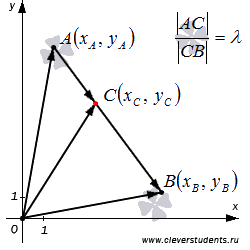
\includegraphics[width=0.25\textwidth]{pict001.png}
\end{wrapfigure}
Мы знаем, что координаты радиус-вектора точки равны
соответствующим координатам этой точки, поэтому, $|\overline{OA}|=(x_a,y_a)$ и $\overline{OB}=(x_b,y_b)$. Найдем координаты вектора $\overline{OC}$,
которые будут равны искомым координатам точки $C$,
делящей отрезок $AB$ в заданном отношении $\lambda$.

В силу операции сложения векторов можно записать
равенства $\overline{OC}=\overline{OA}+\overline{AC}$ и $\overline{OB} = \overline{OC} +\overline{CB}\,\Leftrightarrow\,\overline{CB} = \overline{OB} - \overline{OC}$. Их мы используем в следующем абзаце.

Так как точка $С$ делит отрезок $АВ$ в соотношении $\lambda$, то $|\overline{AC}|=\lambda\cdot|\overline{CB}|$. Векторы $\overline{AC}$ и $\overline{CB}$ лежат на одной прямой и имеют одинаковое направление, а выше мы отметили, что $\lambda>0$, поэтому, по определению операции умножения вектора на число, справедливо равенство $\overline{AC} = \lambda\cdot\overline{CB}$ . Подставив в него $\overline{CB} = \overline{OB} - \overline{OC}$ , имеем $\overline{AC} = \lambda\cdot(\overline{OB} - \overline{OC})$.
Тогда равенство $\overline{OC} = \overline{OA} +\lambda\cdot(\overline{OB} - \overline{OC})$, откуда в силу свойств операций над векторами получаем:
$$ \overline{OC} =\frac{1}{1+\lambda}\cdot(\overline{OA}+\lambda\cdot\overline{OB}) $$
Осталось вычислить координаты вектора $\overline{OC} =\frac{1}{1+\lambda}\cdot(\overline{OA}+\lambda\cdot\overline{OB})$, выполнив необходимые операции над векторами $\overline{OA}$ и $\overline{OB}$ в координатах. Так как $\overline{OA}=(x_a,y_a)$ и $\overline{OB}=(x_b,y_b)$, то $\overline{OA}+\lambda\cdot\overline{OB}=(x_a+\lambda\cdot x_b,\,y_a+\lambda\cdot y_b)$, а следовательно:
$$ \overline{OC}= \frac{1}{1+\lambda}\cdot(\overline{OA}+\lambda\cdot\overline{OB}) = \bigg(\frac{x_a+\lambda\cdot x_b}{1+\lambda},\,\frac{y_a+\lambda\cdot y_b}{1+\lambda}\bigg)$$
\newpage
\section{Полярная система координат на плоскости и её связь с декартовой. Преобразования декартовой системы координат на плоскости и в пространстве (поворот, параллельный перенос)}
\subsection{Полярная система координат}
\subsubsection{Определение}
\textbf{Полярная система координат} определяется заданием некоторой точки $O$, называемой полюсом, исходящего из этой точки луча $OA$ (обозначается также и как $Ox$), называемого полярной осью, и масштаба для изменения длин. Кроме того, при задании полярной системы координат должно быть определено, какие повороты вокруг точки O считаются положительными (на чертежах обычно положительными считаются повороты против часовой стрелки).
\subsubsection{Связь полярных координат с декартовыми координатами}
Установим связь между полярными координатами точки и её декартовыми координатами. Будем предполагать, что начало декартовой прямоугольной системы координат находится в полюсе, а положительная полуось абсцисс совпадает с полярной осью. Пусть точка $M$ имеет декартовы координаты $x$ и $y$ и полярные координаты $\rho$ и $\varphi$. Тогда $x=\rho\cdot\cos(\varphi);\:y=\rho\cdot\sin(\varphi)$.
\subsection{Преобразования прямоугольной ДСК}

\subsubsection{Параллельный перенос}
    \begin{wrapfigure}{l}{0.3\textwidth}
        \centering
        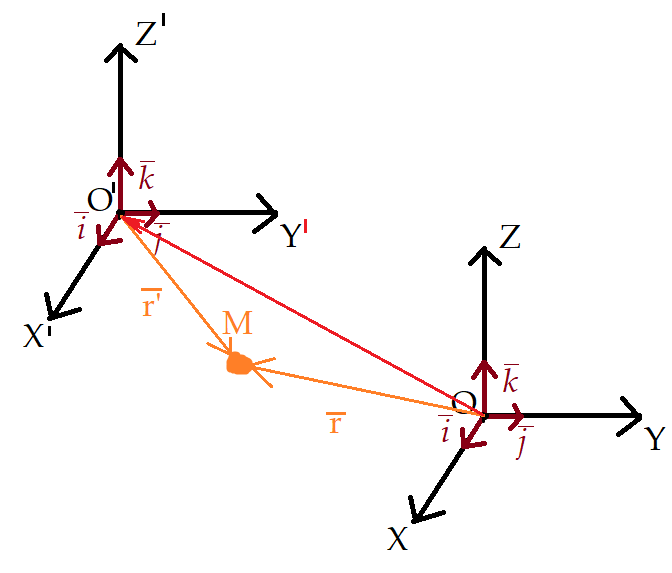
\includegraphics[scale=0.3]{pic33.png}
    \end{wrapfigure}
    $\overline{OO'}=(x_0,y_0,z_0)=O'$ -- координаты нового центра СК в старых координатах.

    $\overline{r}=(x,y,z)=M=\overline{OM}$

    $\overline{r}==\overline{OO'}+\overline{r'}$

    $ \overline{r}'=(x',y'z') $

    $$ \begin{cases}x=x_0+x'\\y=y_0+y'\\z=z_0+z' \end{cases}$$
    lalalalala...

    lallalalala!

\newpage
\subsubsection{Поворот на плоскости}
    \begin{wrapfigure}{l}{0.3\textwidth}
        \centering
        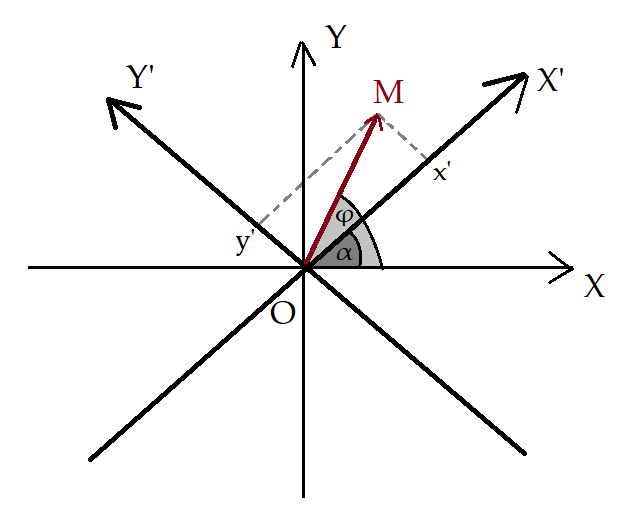
\includegraphics[scale=0.3]{pic34.png}
    \end{wrapfigure}
    $$ \begin{cases} x'=r\cos\varphi \\y'=r\sin\varphi \end{cases}$$
    $$ \begin{cases} x=r\cos(\varphi+\alpha) \\ y=r\sin(\varphi+\alpha) \end{cases} $$
    $$ \begin{cases}x=x'\cdot\cos\alpha-y'\cdot\sin\alpha\\y=x'\cdot\sin\alpha+y'\cdot\cos\alpha\end{cases}\,\Leftrightarrow\,\begin{cases} x'=\cos\alpha x +\sin\alpha y\\y'=-\sin\alpha x+\cos\alpha y \end{cases}$$

    lalala

\subsubsection{Поворот в пространстве}

    Матрица поворота
    \textit{ух ёпт, поехали выводить это говно}

    Базисные векторы в изначальной ДСК -- $\overline{i},\,\overline{
    j},\,\overline{k}$. Базисные вектора в новой системы координат -- $\overline{e}_1,\,\overline{e}_2,\,\overline{e}_3$. То есть, $\overline{r}=x\overline{i}+y\overline{j}+z\overline{k}=x'\overline{e}_1+y'\overline{e}_2+z'\overline{e}_3 $. Вектора $\overline{e}_1=(\cos\alpha_1,\cos\beta_1,\cos\gamma_1)^T,\,\overline{e}_2=(\cos\alpha_2,\cos\beta_2,\cos\gamma_2)^T,\,\overline{e}_3=(\cos\alpha_3,\cos\beta_3,\cos\gamma_3)^T$, где $\alpha_1,\,\beta_1,\,\gamma_1$ -- углы между вектором $\overline{e}_1$ и соответственно осями $Ox,\,Oy,\,Oz$ (остальные углы аналогично). Тогда
    $$ \begin{cases} x=x'\cos\alpha_1+y'\cos\alpha_2+z'\cos\alpha_3 \\ y=x'\cos\beta_1+y'\cos\beta_2+z'\cos\beta_3 \\ z=x'\cos\gamma_1+y'\cos\gamma_2+z'\cos\gamma_3 \end{cases} $$
    Ну или матрциа поворота
    \[
    \begin{bmatrix}
    x \\
    y \\
    z
    \end{bmatrix}
    =
    \begin{bmatrix}
    \cos\alpha_1 & \cos\alpha_2 & \cos\alpha_3 \\
    \cos\beta_1 & \cos\beta_2 & \cos\beta_3 \\
    \cos\gamma_1 & \cos\gamma_2 & \cos\gamma_3
    \end{bmatrix} \cdot
    \begin{bmatrix}
    x' \\
    y' \\
    z'
    \end{bmatrix}
    \]

\newpage
\section{Скалярное произведение векторов и его свойства. Выражение координат вектора через скалярное произведение. Критерий ортогональности векторов. Формула скалярного произведения в координатном представлении.}
\subsection{Скалярное произведение векторов}
\subsubsection{Определение}
\textbf{Скалярное произведение двух векторов $\overline{a}$ и $\overline{b}$} -- скалярная величина, равная
произведению модулей этих векторов, умноженному на косинус угла между ними:
$$\overline{a}\cdot \overline{b} = |\overline{a}|\cdot |\overline{b}| \cos\alpha$$
\subsubsection{Координатное представление формулы}
Скалярная величина, равная сумме попарного произведения координат векторов $\overline{a}$ и $\overline{b}$: $$\overline{a}\cdot\overline{b}=a_1\cdot b_1+a_2\cdot b_2+a_3\cdot b_3$$
\subsubsection{Свойства}
\begin{enumerate}
    \item Симметричность или коммутативность: $\overline{a}\cdot\overline{b}=\overline{b}\cdot\overline{a}$
    \item Аддитивность (линейность): $(\overline{a}_1+\overline{a}_2)\cdot\overline{b}=\overline{a}_1\cdot\overline{b}+\overline{a}_2\cdot\overline{b}$
    \item Однородность: $(\lambda\cdot\overline{a})\cdot\overline{b}=\lambda\cdot(\overline{a}\cdot\overline{b})$

    2 и 3 свойства дают линейность по первому аргументу, а в силу свойства 1 -- ещё и линейность по второму.
    \item Произведение вектора самого на себя: $\overline{a}\cdot\overline{a}\geqslant 0;\;\overline{a}\cdot\overline{a}=|\overline{a}|^2$
\end{enumerate}
\subsubsection{Критерий ортогональности векторов}
$$ \overline{a},\,\overline{b}\neq 0,\,\overline{a}\cdot\overline{b}=0\,\Leftrightarrow\,\overline{a}\perp\overline{b} $$

\newpage
\section{Векторное произведение векторов и его свойства (кроме аддитивности). Критерий коллинеарности векторов. Формула векторного произведения в координатном представлении. Смешанное произведение векторов и его свойства. Доказательство аддитивности векторного произведения. Критерий компланарности векторов. Формула смешанного произведения в координатном представлении. Двойное векторное произведение.}
\subsection{Векторное произведение векторов}
\subsubsection{Определение}
\textbf{Векторным произведением вектора $\overline{a}$ на вектор $\overline{b}$} называется вектор $\overline{c}$, длина которого
численно равна площади параллелограмма построенного на векторах $\overline{a}$ и $\overline{b}$,
перпендикулярный к плоскости этих векторов и направленный так, чтоб наименьшее
вращение от $\overline{a}$ к $\overline{b}$ вокруг вектора осуществлялось против часовой стрелки, если
смотреть с конца вектора $\overline{c}$.
$$\overline{a}\times\overline{b}=[\overline{a},\overline{b}]=|\overline{a}|\cdot|\overline{b}|\cdot\sin\alpha$$
\subsubsection{Левая и правая тройки векторов}
Тройка векторов $\overline{a}$, $\overline{b}$ и  $\overline{c}$ называется \textit{левой}, если поворот от вектора $\overline{a}$ к вектору $\overline{b}$,
видимый с конца третьего вектора $\overline{c}$, осуществляется по ходу часовой стрелки (рис. 1).

Тройка векторов $\overline{a}$, $\overline{b}$ и  $\overline{c}$ называется \textit{правой}, если поворот от вектора $\overline{a}$ к вектору $\overline{b}$,
видимый с конца третьего вектора $\overline{c}$, осуществляется против хода часовой стрелки (рис. 2).
\begin{center}
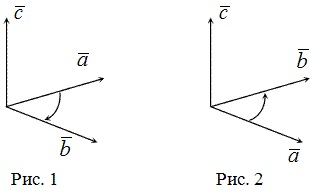
\includegraphics[scale=1.2]{lalala.jpg}
\end{center}
\subsubsection{Свойства}
\begin{enumerate}
    \item \textit{Геометрический смысл векторного произведения}: модуль векторного произведения двух векторов $\overline{a}$ и $\overline{b}$ равен площади параллелограмма, построенного на этих векторах: $S_{par} = [\overline{a} \times \overline{b}]$
    \item Векторное произведения двух не нулевых векторов $\overline{a}$ и $\overline{b}$ равно нулю тогда и только  тогда, когда вектора коллинеарны.
    \item Вектор $\overline{c}$, равный векторному произведению ненулевых векторов $\overline{a}$ и $\overline{b}$, перпендикулярен этим векторам.
    \item Антикоммутативность: $\overline{a} \times \overline{b}=-\overline{b}\times\overline{a}$
    \item Ассоциативность относительно скаляра: $(\lambda\cdot\overline{a}\times\overline{b})=\overline{a}\times(\lambda\cdot\overline{b})=\lambda\cdot(\overline{a}\times\overline{b})$

\end{enumerate}

\subsubsection{Координатное представление}
\[
    \overline{a}\times\overline{b}
    =
    \begin{bmatrix}
    \overline{i} & \overline{j} & \overline{k} \\
    a_1 & a_2 & a_3 \\
    b_1 & b_2 & b_3
    \end{bmatrix}
    = \overline{i}\cdot A_{11}+\overline{j}\cdot A_{12} +\overline{k}\cdot A_{13} =
\]
\[
    =\overline{i}\cdot(a_2\cdot b_3-a_3\cdot b_2)+\overline{j}\cdot(a_1\cdot b_3-a_3\cdot b_1)+\overline{k}\cdot(a_2\cdot b_1-a_1\cdot b_2)
\]
\subsubsection{Свойство аддитивности (линейности)}
 Векторное произведение линейно по каждому аргументу, т.е. для любых векторов и для любого числа $\lambda$ выполняется
 $$ [\overline{a}_1+\overline{a}_2,\overline{b}]=[\overline{a}_1,\overline{b}]+[\overline{a}_2,\overline{b}] $$
 $$ [\lambda\cdot\overline{a},\overline{b}]=[\overline{a},\lambda\cdot\overline{b}]=\lambda\cdot[\overline{a},\overline{b}] $$

\textbf{Доказательство}

Пусть $\overline{c}=[\overline{a}_1+\overline{a}_2,\overline{b}]-[\overline{a}_1,\overline{b}]-[\overline{a}_2,\overline{b}]$. Докажем, что он равен нулю, доказав, что его скалярный квадрат равен нулю, т.е. что $(\overline{c},\overline{c})=0$. (Применим свойства линейности скалярного произведения и определение смешанного произведения\footnote{см. п. 4.2})
$$ (\overline{c},\overline{c})=([\overline{a}_1+\overline{a}_2]-[\overline{a}_1,\overline{b}]-[\overline{a}_2,\overline{b}],\overline{c})=([\overline{a}_1+\overline{a}_2,\overline{b}],\overline{c})-([\overline{a}_1,\overline{b}],\overline{c})-([\overline{a}_2,\overline{b}],\overline{c})= $$
$$ =(\overline{a}_1+\overline{a}_2,\overline{b},\overline{c})-(\overline{a}_1,\overline{b},\overline{c})-(\overline{a}_2,\overline{b},\overline{c}) =-(\overline{c},\overline{b},\overline{a}_1+\overline{a}_2)+(\overline{c},\overline{b},\overline{a}_1)+(\overline{c},\overline{b},\overline{a}_2)=$$
$$ =-([\overline{c},\overline{b}],\overline{a}_1+\overline{a}_2)+([\overline{c},\overline{b}],\overline{a}_1)+([\overline{c},\overline{b}],\overline{a}_2)=0 $$
\n
\n
\n
\subsection{Смешанное произведение векторов}
\subsubsection{Определение}
\textbf{Смешанное произведение векторов} — скалярное произведение вектора $\overline{a}$ на
векторное произведение векторов  $\overline{b}$ и $\overline{c}$. $$(\overline{a},\overline{b},\overline{c})=\overline{a}\cdot(\overline{b}\times\overline{c})=\overline{a}\cdot\overline{b}\cdot\overline{c}$$
\subsubsection{Свойства}
\begin{itemize}
    \item  \textit{Геометрический смысл смешанного произведения}: модуль смешанного произведения трех векторов $\overline{a}$, $\overline{b}$ и  $\overline{c}$ равен объёму параллелепипеда, образованного этими векторами: $V_{par}=|\overline{a}\cdot(\overline{b}\times\overline{c})|$ ($V>0$, если $\overline{a},\overline{b},\overline{c}$ - правая тройка, если левая тройка -- $V<0$)
    \item $(\overline{a},\overline{b},\overline{c})=-(\overline{a},\overline{c},\overline{b})$
\end{itemize}
\subsubsection{Критерий компланарности векторов}
Если смешанное произведения трех ненулевых векторов равно нулю, то эти вектора компланарные.
\subsubsection{Двойное векторное произведение}
$$ \overline{a}\times(\overline{b}\times\overline{c})=\overline{b}\cdot(\overline{a}\cdot\overline{c})-\overline{c}\cdot(\overline{a}\cdot\overline{b}) = \overline{d}=(a_2\cdot b_1\cdot c_2,\,-a_1\cdot b_1\cdot c_2,\, 0) $$

\newpage
\section{Теорема об общем уравнении прямой на плоскости. Различные способы задания прямой на плоскости: общее уравнение прямой, уравнение в отрезках, через точку и нормаль, параметрическое, каноническое и нормальное уравнения прямой. Вычисление расстояния от точки до прямой. Полярное уравнение прямой. Взаимное расположение прямых на плоскости.}
\subsection{Уравнения, задающие прямую на плоскости}
\subsubsection{Общее уравнение прямой}
Уравнение вида $Ax + By + C = 0$ ($A$ и $B$ одновременно не равны нулю) называется \textbf{общим уравнением прямой на плоскости}. Общее уравнение прямой называется \textit{полным}, если все числа $A$, $B$ и $C$ отличны от нуля, в противном случае общее уравнение прямой называется \textit{неполным}.

\textbf{ТЕОРЕМА}. Всякое уравнение первой степени вида $Ax+By+C=0$, где $A$, $B$ и $C$ – некоторые действительные числа, причем А и В одновременно не равны нулю, задает прямую линию в прямоугольной системе координат $Oxy$ на плоскости, и любая прямая в прямоугольной системе координат $Oxy$ на плоскости задается уравнением вида $Ax+By+C=0$ при некотором наборе значений $A$, $B$ и $C$.

\textbf{Доказательство}

I. Докажем сначала, что уравнение вида $Ax+By+C=0$ задает прямую на плоскости.

Пусть координаты точки $M_0(x_0,y_0)$ удовлетворяют уравнению $Ax+By+C=0$, то есть, $Ax_0+By_0+C=0$. Вычтем из левой и правой частей уравнения $Ax+By+C=0$ соответственно левую и правую части равенства $Ax_0+By_0+C=0$, при этом получаем уравнение вида $A(x-x_0)+B(y-y_0)$, которое эквивалентно $Ax+By+C=0$.

Уравнение $A(x-x_0)+B(y-y_0)$ представляет собой необходимое и достаточное условие перпендикулярности двух векторов $\overline{n}=(A,B)$ и $\overline{M_0M}=(x-x_0,y-y_0)$. То есть, множество всех точек $M(x,y)$ определяет в прямоугольной системе координат $Oxy$ прямую линию, перпендикулярную направлению вектора $\overline{n}=(A,B)$. Если бы это было не так, то векторы $\overline{n}=(A,B)$ и $\overline{M_0M}=(x-x_0,y-y_0)$ не были бы перпендикулярными и равенство $A(x-x_0)+B(y-y_0)$ не выполнялось бы.
\begin{center}
    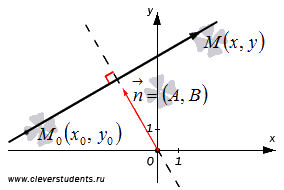
\includegraphics[scale=0.5]{pict001 (1).png}
\end{center}
Таким образом, уравнение $A(x-x_0)+B(y-y_0)$ задает прямую линию в прямоугольной декартовой системе координат $Oxy$ на плоскости, следовательно, эквивалентное ему уравнение вида $Ax+By+C=0$ задает эту же прямую. На этом первая часть теоремы доказана.

II. Теперь докажем, что всякая прямая в прямоугольной системе координат $Oxy$ на плоскости определяется уравнением первой степени вида $Ax+By+C=0$.

Пусть в прямоугольной системе координат $Oxy$ на плоскости задана прямая $a$, проходящая через точку $M_0(x_0,y_0)$, $\overline{n}=(A,B)$ -- нормальный вектор прямой $a$, и пусть $M(x,y)$ -- плавающая точка этой прямой. Тогда векторы $\overline{n}=(A,B)$ и $\overline{M_0M}=(x-x_0,y-y_0)$ перпендикулярны, следовательно, их скалярное произведение равно нулю, то есть, $(\overline{n},\overline{M_0M})=A(x-x_0)+B(y-y_0)=0$. Полученное равенство можно переписать в виде  $Ax+By-Ax_0-By_0=0$. Если принять $C=-Ax_0-By_0$, то получим уравнение $Ax+By+C=0$, которое соответствует прямой $a$.
\subsubsection{Уравнение в отрезках}
\textbf{Уравнение в отрезках} прямой, пересекающей ось $Ox$  в точке $(a,0)$ и ось $Oy$  в точке $(0,b)$
$$ \frac{x}{a}+\frac{y}{b}=1\:(a\neq 0,\, b\neq 0) $$
\subsubsection{Векторное уравнение}
\textbf{Векторное уравнение прямой} в параметрической форме $\overline{r} = \overline{r}_0 + \overline{a}\cdot t, \overline{a} \neq 0$, где $\overline{a}$ — направляющий вектор прямой, $\overline{r}_0$ -- радиус-вектор некоторой точки прямой.
\subsubsection{Параметрическое уравнение}
Прямая линия на плоскости может быть задана \textbf{параметрическим уравнением} прямой: $x = x_0 + \alpha\cdot t, y = y_0 + \beta\cdot t$ (просто разложили векторное уравнение прямой по координатам $x$ и $y$), где числа $\alpha,\,\beta$ не равны нулю одновременно и являются компонентами направляющего вектора прямой -- ненулевого вектора, лежащего на прямой.
\subsubsection{Каноническое уравнение}
Если $\alpha\neq0,\,\beta\neq0$, то после исключения из уравнений прямой в параметрической форме параметра $t$ уравнение прямой приводятся к \textbf{канонической форме}:
$$ \frac{x-x_0}{\alpha}=\frac{y-y_0}{\beta} $$
\subsubsection{Нормальное векторное уравнение}
$(\overline{r} - \overline{r}_0, \overline{n}) = 0, n \neq 0$, где $\overline{n}$ -- вектор нормали к прямой, $\overline{r}_0$ -- радиус вектор
фиксированной точки, $\overline{r}$ -- радиус-вектор любой точки прямой. Это уравнение также можно записать в форме $(\overline{r}, \overline{n}) = D, \overline{n} \neq 0$, или в форме $x\cdot\cos\alpha+y\cdot\sin\alpha-P=0$, где $\alpha$ -- угол между нормалью $\overline{n}$ и осью $Ox$, a $P$ -- проекция радиус-вектора $\overline{r}$ на вектор нормали.
\newline
\newpage
\begin{center}
    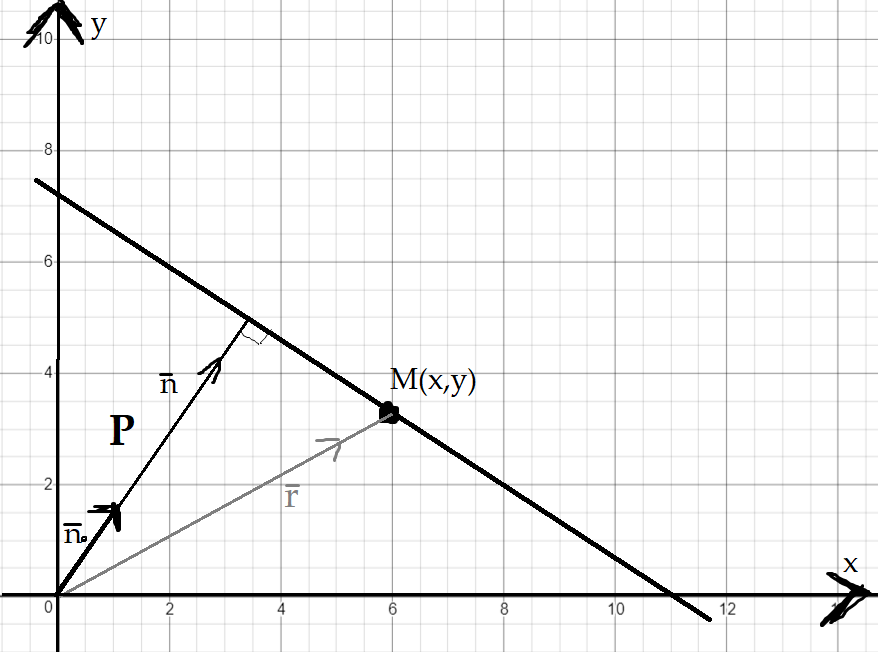
\includegraphics[scale=0.5]{pic.png}
\end{center}
\begin{wrapfigure}{l}{0.3\textwidth}
    \centering
    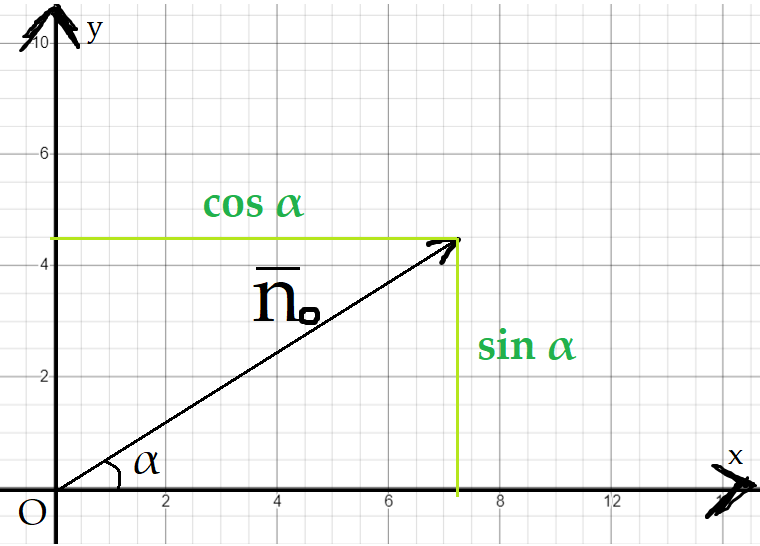
\includegraphics[width=0.25\textwidth]{pci2.png}
\end{wrapfigure}

Расстояние от точки $O$ до прямой $L$ равняется $P$, что, в свою очередь, является проекцией радиус-вектора $\overline{r}$ на орт-вектор нормали $\overline{n}_0$. Координаты вектора $\overline{n}_0=(\cos\alpha,\sin\alpha)$, где $\alpha$ -- угол между осью $Ox$ и орт-вектором $\overline{n}_0$.

Скалярное произведение векторов $(\overline{r},\overline{n}_0)$ равняется $P$ и так же равняется $x\cdot\cos\alpha+y\cdot\sin\alpha$. Следовательно, $x\cdot\cos\alpha+y\cdot\sin\alpha-P=0$ -- нормальное уравнение прямой.

Чтобы привести от общего вида к нормальному, надо поделить на $\pm\sqrt{A^2+B^2}$.
$$ \frac{A}{\pm\sqrt{A^2+B^2}}x+\frac{B}{\pm\sqrt{A^2+B^2}}y+\frac{C}{\pm\sqrt{A^2+B^2}}=0\,\Leftrightarrow\, $$
$$\,\Leftrightarrow\,\frac{A}{\pm\sqrt{A^2+B^2}} = \cos\alpha,\,\frac{B}{\pm\sqrt{A^2+B^2}}=\sin\alpha, \frac{C}{\pm\sqrt{A^2+B^2}}=-P\,\Leftrightarrow$$
$$ \Leftrightarrow\,x\cdot\cos\alpha+y\cdot\sin\alpha-P=0$$
\newpage
\subsubsection{Полярное уравнение}
Полярное уравнение в полярной системе координат задаётся через радиус-вектор $\overline{r}$, углом $\varphi$ между радиус-вектором и осью $Ox$, проекцией $P$ радиус-вектора на нормаль прямой и углом $\alpha$ между нормалью и осью $Ox$.
$$ \begin{cases} x=\overline{r}\cdot\cos\varphi \\y=\overline{r}\cdot\sin\varphi \end{cases}\,\Leftrightarrow\;\overline{r}=\frac{P}{cos(\varphi-\alpha)} $$
\begin{center}
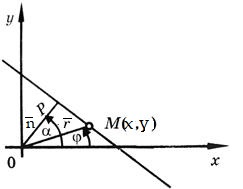
\includegraphics[scale=0.8]{2.jpg}
\end{center}
\subsection{Расстояние от точки до прямой}
Расстояние от точки до прямой равно длине перпендикуляра, опущенного из точки на прямую. Если задано уравнение прямой $Ax + By + C = 0$, то расстояние от точки $M(x,y)$ до прямой можно найти, используя следующую формулу:
$$ d=\frac{|Ax+By+C|}{\sqrt{A^2+B^2}} $$
\textbf{Доказательство}

Пусть $P$ -- точка с координатами$(x_0 , y_0 )$ и пусть
исходная прямая имеет уравнение $ax + by + c = 0$. Пусть $Q = ( x_1 , y_1 )$ — любая точка на
прямой и $\overline{n}$ -- вектор $( a , b )$ с началом в точке $Q$. Вектор $\overline{n}$ перпендикулярен прямой, и
расстояние $d$ от точки $P$ до прямой равно длине ортогональной проекции $\overline{QP }$ на $\overline{n}$.
Длина этой проекции равна:
$$ d = \frac{|\overline{QP}\cdot\overline{n}|}{|\overline{n}|} $$
Теперь
$\overline{QP} = (x_0 - x_1, \,y_0 - y_1)$, так что $\overline{QP}\cdot\overline{n} = a\cdot(x_0 - x_1) + b\cdot(y_0 - y_1)$ и $|\overline{n}| = \sqrt{a^2+b^2}$. Тогда
$$ d = \frac{|a\cdot(x_0 - x_1) + b\cdot(y_0 - y_1)|}{\sqrt{a^2+b^2}}$$
Поскольку $Q$ лежит на заданной прямой, $ax_1 + by_1 + c = 0\,\Rightarrow\, c = - ax_1 - by_1$, а тогда если
раскрыть числитель нашей дроби и заменить $- ax_1 - by_1$ на $c$, то получится:
$$ d=\frac{|ax_0+by_0+c|}{\sqrt{a^2+b^2}} $$
\newpage
\subsection{Взаимное расположение прямых на плоскости}
Две прямые $L_1=A_1x+B_1y+C_1,\,L_2=A_2x+B_2y+C_2;\;\overline{n}_1=(A_1,B_1),\,\overline{n}_2=(A_2,B_2);\;L_1\cap L_2=M_0;\; M_1\in L_1,\, M_2\in L_2$
\subsubsection{Параллельны или совпадают}
    $$ L_1 ||\,L_2\,\Leftrightarrow\,\overline{n}_1||\,\overline{n}_2\,\Leftrightarrow\,\frac{A_1}{A_2}=\frac{B_1}{B_2} $$
    Совпадают, если $\frac{C_1}{C_2}$ равно описанному выше равенству.
    $$ d(L_1,L_2)=\frac{|\overline{s}_1\cdot\overline{M_1M_2}|}{|\overline{s}_2|} $$
\subsubsection{Пересекаются}
    $$ L_1\cap L_2\,\Leftrightarrow\,\overline{n}_1\nparallel\overline{n}_2\,\Leftrightarrow\, \frac{A_1}{A_2}\neq\frac{B_1}{B_2}$$
\subsubsection{Перпендикулярны (подслучай п.5.3.2)}
    $$ L_1:\:y=k_1\cdot x+b_1 $$
    $$ L_2:\:y=k_2\cdot x+b_2 $$
    $$ L_1\perp L_2\,\Leftrightarrow\, k_1\cdot k_2=-1 $$

\newpage
\section{Теорема об общем уравнении плоскости в пространстве. Различные способы задания плоскости в пространстве: общее уравнение плоскости, уравнение в отрезках, через точку и нормаль, нормальное уравнение плоскости. Вычисление расстояния от точки до плоскости. Взаимное расположение плоскостей в пространстве}
\subsection{Уравнения плоскости в пространстве}
\subsubsection{Общее уравнение}
\textbf{Общее уравнение плоскости} : $Ax + By + Cz + D = 0$ ($A$, $B$, $C$ одновременно не равны
нулю). Вектор с координатами $\overline{n}=(A, B, C)$ является \textit{нормальным вектором} к плоскости.

$\bullet$ Пусть нам дана прямоугольная система координат $Oxyz$ в трехмерном пространстве, уравнением плоскости в заданной системе координат будет такое уравнение с тремя неизвестными $x$, $y$, $z$, которому отвечали бы координаты всех точек этой плоскости и не отвечали бы координаты никаких прочих точек. Иначе говоря, подставив в уравнение плоскости координаты некоторой точки этой плоскости, получаем тождество. $\bullet$

\textbf{ТЕОРЕМА}. Всякое уравнение вида $Ax+By+Cz+D=0$, где $A$, $B$, $C$ и $D$ -- некоторые действительные числа, причем $A$, $B$ и $C$ одновременно не равны нулю, определяет плоскость в прямоугольной системе координат $Oxyz$ в трехмерном пространстве, и всякая плоскость в прямоугольной системе координат $Oxyz$ в трехмерном пространстве может быть задана уравнением вида $Ax+By+Cz+D=0$.

\textbf{Доказательство}

\begin{wrapfigure}{l}{0.3\textwidth}
    \centering
    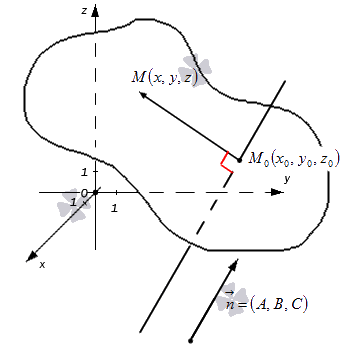
\includegraphics[width=0.25\textwidth]{image015.png}
\end{wrapfigure}
I. Первая часть теоремы гласит, что любую заданную плоскость возможно описать уравнением вида $Ax+By+Cz+D=0$. Допустим, задана некоторая плоскость и точка $M_0(x_0,y_0,z_0)$, через которую эта плоскость проходит. Нормальным вектором этой плоскости является $\overline{n}=(A,B,C)$. Приведем доказательство, что указанную плоскость в прямоугольной системе координат $Oxyz$
задает уравнение $Ax+By+Cz+D=0$.

Возьмём произвольную точку заданной плоскости $V(x,y,z)$. В таком случае векторы $\overline{n}=(A,B,C)$ и $\overline{M_0M}=(x-x_0,y-y_0,z-z_0)$ будут перпендикулярны друг другу, а значит их скалярное произведение равно нулю: $(\overline{n},\overline{M_0M})=A(x-x_0)+B(y-y_0)+C(z-z_0)=Ax+By+Cz-(Ax_0+By_0+Cz_0)=0$.

Примем $D=-(Ax_0+By_0+Cz_0)$, тогда получим наше исходное уравнение $Ax+By+Cz+D=0$, что и требовалось доказать.

\newpage

II. Во второй части теоремы утверждается, что любое уравнение вида $Ax+By+Cz+D=0$ (при $A,\,B,\,C\neq 0$)
 задает некоторую плоскость в прямоугольной системе координат $Oxyz$
 трехмерного пространства. Докажем это.

В силу того, что $A,\,B,\,C\neq 0$, существует такая точка $M_0(x_0,y_0,z_0)$, координаты которой отвечают уравнению $Ax+By+Cz+D=0$, то есть получим равенство $Ax_0+By_0+Cz_0+D=0$. Отнимем левую и правую части этого равенства от левой и правой частей уравнения $Ax+By+Cz+D=0$, получим $A(x-x_0)+B(y-y_0)+C(z-z_0)=Ax+By+Cz-(Ax_0+By_0+Cz_0)=0$, которое эквивалентно исходному. Докажем, что оно задаёт плоскость.

Данное уравнение представляем собой скалярное произведение векторов $\overline{n}=(A,B,C)$ и $\overline{M_0M}=(x-x_0,y-y_0,z-z_0)$ -- следовательно, в силу равенства нулю, вектора перпендикулярны. Опираясь на утверждение, указанное перед теоремой, возможно утверждать, что при справедливом равенстве $A(x-x_0)+B(y-y_0)+C(z-z_0)=0$ множество точек $M(x,y,z)$ задаёт плоскость, у которой нормальный вектор $\overline{n}=(A,B,C)$. При этом плоскость проходит через точку $M_0$. Иначе говоря, уравнение $A(x-x_0)+B(y-y_0)+C(z-z_0)=0$ задаёт плоскость. Если примем $D=-(Ax_0+By_0+Cz_0)=0$, то получим уравнение $Ax+By+Cz+D=0$, то есть уравнение исходное, что и требовалось доказать.
\subsubsection{Уравнение в отрезках}
Если плоскость пересекает оси $Ox$, $Oy$ и $Oz$ в точках с координатами $(a, 0, 0)$, $(0, b, 0)$ и $(0, 0, с)$, то она может быть найдена, используя формулу уравнения плоскости в отрезках:
$$ \frac{x}{a}+\frac{y}{b}+\frac{z}{c}=1\:(a,b,c\neq0) $$
\subsubsection{Уравнение через точку и вектор нормали}
\begin{wrapfigure}{l}{0.3\textwidth}
    \centering
    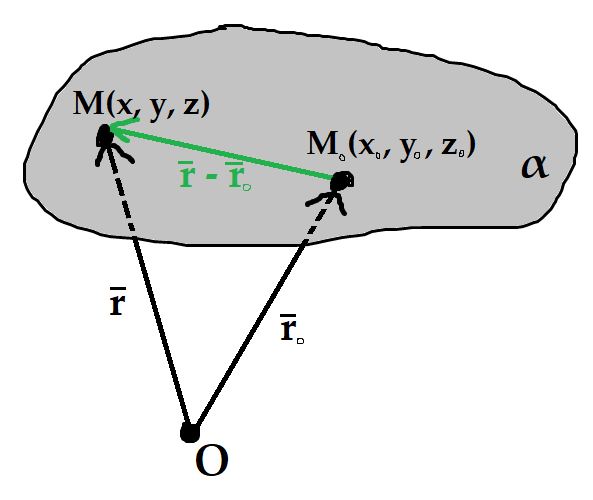
\includegraphics[width=0.25\textwidth]{pic3.png}
\end{wrapfigure}
Уравнение плоскости $Ax+By+Cz+D=0$. Пусть плоскости $\alpha$ принадлежат точки $M(x,y,z)$ и $M_0(x_0,y_0,z_0)$. Вектор нормали $\overline{n}=(A,B,C)$.

Допустим из точки $O$ пространства проведены два радиуса вектора -- $\overline{r}$ к точке $M$ и $\overline{r}_0$ к точке $M_0$. Тогда вектор $\overline{r}-\overline{r}_0$ лежит в плоскости $\alpha$ и перпендикулярен вектору нормали $\overline{n}$. Его координаты $\overline{r}-\overline{r}_0=(x-x_0,y-y_0,z-z_0)$.

$\overline{r}-\overline{r}_0\perp \overline{n}\,\Leftrightarrow\,(\overline{r}-\overline{r}_0,\overline{n})=0\,\Leftrightarrow\,$

$\Leftrightarrow\, A(x-x_0)+B(y-y_0)+C(z-z_0)=0 $

Получили уравнение плоскости через точку и вектор нормали.

\newpage
\subsubsection{Нормальное уравнение}
\begin{center}
    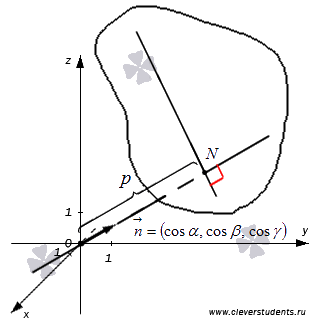
\includegraphics[scale=0.6]{pic4.png}
\end{center}
Всё только в символах, без слов.
$$ \overline{n}_0=\frac{\overline{n}}{|\overline{n}|}\perp \alpha,\,\overline{n}_0=(\cos\alpha,\cos\beta,\cos\gamma),\, M(x,y,z)\in\alpha$$
$$d(O,\alpha) = P,\,P=proection_{\,\overline{n}_0}\overline{r}\,\Leftrightarrow\,(\overline{r},\overline{n}_0)=P\,\Leftrightarrow$$
$$ \Leftrightarrow\,x\cdot\cos\alpha+y\cdot\cos\beta+z\cdot\cos\gamma-P=0 $$
Если обе части уравнения $Ax+By+Cz+D=0$ поделить на $\pm\sqrt{A^2+B^2+C^2}$:
$$ \frac{A}{\pm\sqrt{A^2+B^2+C^2}}\cdot x+\frac{B}{\pm\sqrt{A^2+B^2+C^2}}\cdot y+\frac{C}{\pm\sqrt{A^2+B^2+C^2}}\cdot z +\frac{D}{\pm\sqrt{A^2+B^2+C^2}}=0 \,\Leftrightarrow$$
$$ \Leftrightarrow\,\cos\alpha=\frac{A}{\pm\sqrt{A^2+B^2+C^2}},\,\cos\beta=\frac{B}{\pm\sqrt{A^2+B^2+C^2}},\,\cos\gamma=\frac{C}{\pm\sqrt{A^2+B^2+C^2}},\,-P=\frac{D}{\pm\sqrt{A^2+B^2+C^2}}\,\Leftrightarrow $$
$$ \Leftrightarrow\,x\cdot\cos\alpha+y\cdot\cos\beta+z\cdot\cos\gamma-P=0$$
\newpage
\subsection{Расстояние от точки до плоскости}
\begin{wrapfigure}{l}{0.3\textwidth}
    \centering
    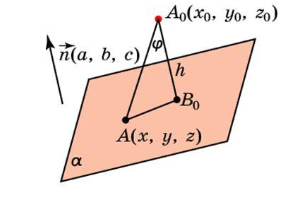
\includegraphics[width=0.25\textwidth]{pic5.png}
\end{wrapfigure}
Расстоянием от точки до плоскости называется длина перпендикуляра, опущенного из данной точки на данную плоскость. Выведем формулу для нахождения расстояния от точки $A_0(x_0,y_0,z_0)$ до плоскости $\alpha$, заданной уравнением $Ax+By+Cz+D=0$.

Пусть $A(x,y,z)\in\alpha$, тогда $\overline{n}=(A,B,C)$ -- вектор нормали данной плоскости.
$$ \cos\varphi=\frac{\overline{n}\cdot\overline{AA}_0}{|\overline{n}|\cdot|\overline{AA}_0|}=\frac{A(x-x_0)+B(y-y_0)+C(z-z_0)}{\sqrt{A^2+B^2+C^2}\cdot|\overline{AA}_0|} $$
Учитывая, что $D=-Ax-By-Cz$ и то, что искомое расстояние равно $|\overline{AA}_0|\cdot\cos\varphi$, получаем
$$ d(A_0,\alpha)=\frac{|Ax_0+By_0+Cz_0+D|}{\sqrt{A^2+B^2+C^2}} $$
\subsection{Взаимное расположение плоскостей в пространстве}
Две плоскости $\alpha_1\::\:A_1x+B_1y+C_1z+D_1=0,\,\alpha_2\::\:A_2x+B_2y+C_2z+D_2=0$
\subsubsection{Плоскости параллельны или совпадают}
\begin{center}
    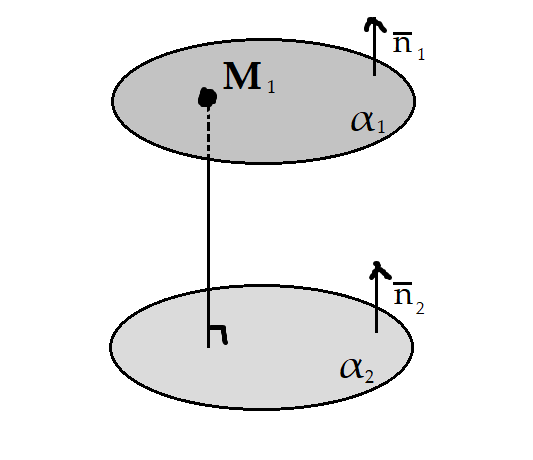
\includegraphics[scale=0.4]{pic6.png}
\end{center}
$$ \alpha_1||\alpha_2\,\Leftrightarrow\,\overline{n}_1||\overline{n}_2\,\Leftrightarrow\,\frac{A_1}{A_2}=\frac{B_1}{B_2}=\frac{C_1}{C_2},\,d(\alpha_1,\alpha_2)=d(M_1,\alpha_2) $$
Чтобы плоскости совпадали:
$$ \frac{A_1}{A_2}=\frac{B_1}{B_2}=\frac{C_1}{C_2}=\frac{D_1}{D_2} $$
\subsubsection{Плоскости пересекаются}
\begin{center}
    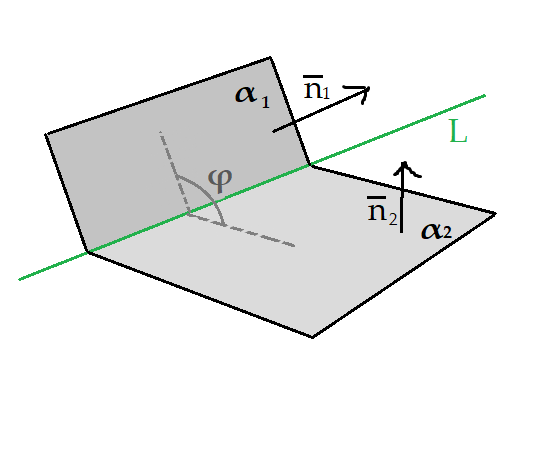
\includegraphics[scale=0.4]{pic7.png}
\end{center}
$$ \alpha_1\cap\alpha_2=L,\,\varphi=\angle(\alpha_1,\alpha_2)=\angle(\overline{n}_1,\overline{n}_2) $$
$$ \alpha_1\cap\alpha_2\,\Leftrightarrow\,\bigg(\frac{A_1}{A_2}\neq\frac{B_1}{B_2}\bigg)\,\lor\,\bigg(\frac{B_1}{B_2}\neq\frac{C_1}{C_2}\bigg)\,\lor\,\bigg(\frac{C_1}{C_2}\neq\frac{A_1}{A_2}\bigg) $$
Угол между плоскостями
$$ \cos\varphi=\frac{\overline{n}_1\cdot\overline{n}_2}{|\overline{n}_1|\cdot|\overline{n}_2|} $$
\newpage
\section{Я ЗАДОЛБАЛАСЬ}
\newpage
\section{Два способа задания прямой в пространстве (переход от одного способа задания к другому). Взаимное расположение прямой и плоскости в пространстве. Взаимное расположение прямых в пространстве, вычисление расстояния между прямыми. Задача о поиске общего перпендикуляра скрещивающихся прямых. Задача о поиске точки симметричной относительно заданной прямой (плоскости), уравнение плоскости через определитель.}
\subsection{Два способа задания прямой в пространстве}
\subsubsection{Пересечение плоскостей}
$$ \begin{cases}A_1x+B_1y+C_1z+D_1=0\:\::\:\alpha_1,\,\overline{n}_1=(A_1,B_1,C_1)\\A_2x+B_2y+C_2z+D_2=0\:\::\:\alpha_2,\,\overline{n}_2=(A_2,B_2,C_2) \end{cases} \Leftrightarrow\:L=\alpha_1\cap\alpha_2 $$
\begin{center}
    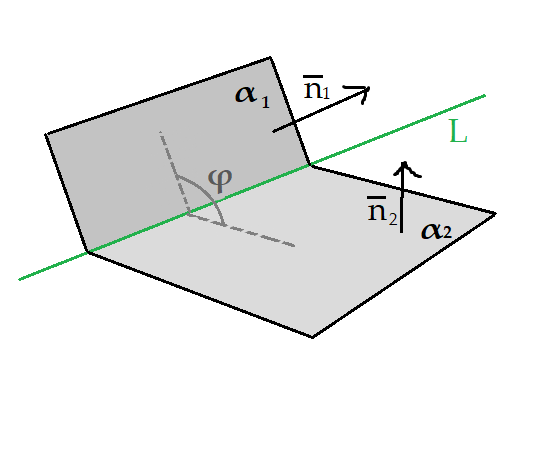
\includegraphics[scale=0.4]{pic7.png}
\end{center}
\subsubsection{Каноническое и параметрическое уравнения}
\begin{wrapfigure}{l}{0.3\textwidth}
    \centering
    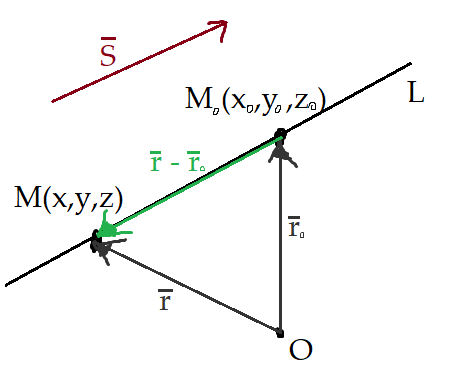
\includegraphics[width=0.25\textwidth]{pic8.png}
\end{wrapfigure}
$M_0\in L,\,\overline{s}\,||\,L,\,\overline{s}=(l,m,n)$

($\overline{r}-\overline{r}_0)\,||\,\overline{s}\,\Leftrightarrow\,\overline{r}-\overline{r}_0=t\cdot\overline{s} $

Если подставить все координаты, то получим формулу в \textbf{параметрическом виде}:

$$ \begin{cases}x=x_0+t\cdot l\\y=y_0+t\cdot m\\z=z_0+t\cdot n \end{cases} $$

Выразив $t$, получим в \textbf{каноническом виде}:
$$ \frac{x-x_0}{l}=\frac{y-y_0}{m}=\frac{z-z_0}{n}=t $$
\newpage
\subsubsection{Переход от первого способа ко второму}
\begin{center}
    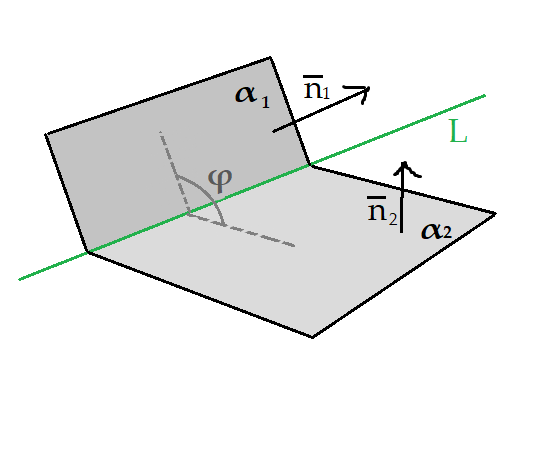
\includegraphics[scale=0.4]{pic7.png}
\end{center}
$$ \begin{cases}A_1x+B_1y+C_1z+D_1=0\:\::\:\alpha_1,\,\overline{n}_1=(A_1,B_1,C_1)\\A_2x+B_2y+C_2z+D_2=0\:\::\:\alpha_2,\,\overline{n}_2=(A_2,B_2,C_2) \end{cases}$$
$$ \overline{s}\perp\overline{n}_1,\,\overline{s}\perp\overline{n}_2\,\Rightarrow\,\overline{s}=\overline{n}_1\times\overline{n}_2 $$
Ищем точку $M_0(x_0,y_0,z_0)\in L$, принадлежащую так же данным двум плоскостям.
\begin{enumerate}
    \item Предположим, что координаты $M_0(0,y_0,z_0)$. Решим систему уравнений:
    $$ \begin{cases}B_1y_0+C_1z_0+D_1=0\\B_2y_0+C_2z_0+D_2=0 \end{cases} $$
    Если есть решения, то точка $M_0$ нам подходит, можем составить каноническое и параметрическое уравнения.

    Если решений нет, то прямая $L\,||Oyz$, смотрим $M_0(x_0,0,z_0)$
    \item аналогично, если подставив координаты точки $M_0(x_0,0,z_0)$ в исходную систему и если решения есть, то точка подходит; если решений нет, то $L\,||Oxz$, смотрим точку $M_0(x_0,y_0,0)$
    \item Если точки $M_0(0,y_0,z_0)$ и $M_0(x_0,0,z_0)$ не подошли, то точка $M_0(x_0,y_0,0)$ обязана подойти.
\end{enumerate}
\subsubsection{Переход от второго способа к первому}
Преобразуем данную систему, это изи.
$$ \begin{cases}(x-x_0)\cdot m=(y-y_0)\cdot l\:\::\:\alpha_1\\(x-x_0)\cdot n=(z-z_0)\cdot l\:\::\:\alpha_2\end{cases} $$
\newpage
\subsection{Взаимное расположение прямой и плоскости в пространстве}
Плоскость $\alpha\::\:Ax+By+Cz+D=0$, прямая $L\::\:\overline{s}=(l,m,n),\,M_0(x_0,y_0,z_0)$
\subsubsection{Прямая параллельна плоскости}
$$ L\,||\alpha\,\Leftrightarrow\,\overline{n}\perp\overline{n}\,\Leftrightarrow\,(\overline{s},\overline{n})=0\,\Leftrightarrow\,Al+Bm+Cn=0$$
Если прямая принадлежит плоскости:
$$ \begin{cases}Al+Bm+Cn=0\\Ax_0+By_0+Cz_0+D=0\end{cases} $$
\subsubsection{Прямая пересекает плоскость}
\begin{center}
    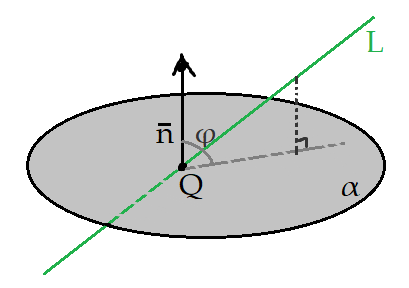
\includegraphics[scale=0.4]{pic9.png}
\end{center}
$$ L\cap\alpha=Q\,\Leftrightarrow\,\overline{n}\not\perp\overline{s}\,\Leftrightarrow\,Al+Bm+Cn\neq0 $$
$$ \angle(L,\alpha)=\varphi=90^{\circ} -\angle(L,\overline{n})$$
$$ \sin\varphi=\cos(\angle(\overline{n},\overline{s}))=\frac{(\overline{n},\overline{s})}{|\overline{n}|\cdot|\overline{s}|} $$
\subsection{Взаимное расположение прямых в пространстве}
Две прямые $L_1\::\:\overline{s}_1=(l_1,m_1,n_1),\:M_1(x_1,y_1,z_1),\:\:L_2\::\:\overline{s}_2=(l_2,m_2,n_2)\,\:M_2(x_2,y_2,z_2)$
\subsubsection{Прямые параллельны или совпадают}
$$ L_1\,||L_2\,\Leftrightarrow\,\overline{s}_1\,||\overline{s}_2\,\Leftrightarrow\,\frac{l_1}{l_2}=\frac{m_1}{m_2}=\frac{n_1}{n_2} $$
$$ d=dist(L_1,L_2) $$
\begin{center}
    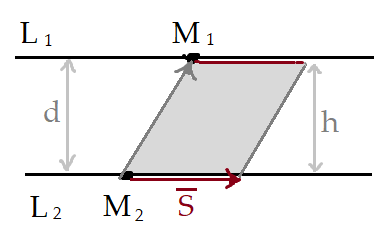
\includegraphics[scale=0.4]{pic10.png}
\end{center}
$$ d=h=\frac{|\overline{s}\cdot\overline{M_1M}_2|}{|\overline{s}|} $$
Если прямые совпадают, то $dist(L_1,L_2)=0$
\subsubsection{Прямые пересекаются или скрещиваются}
\begin{center}
    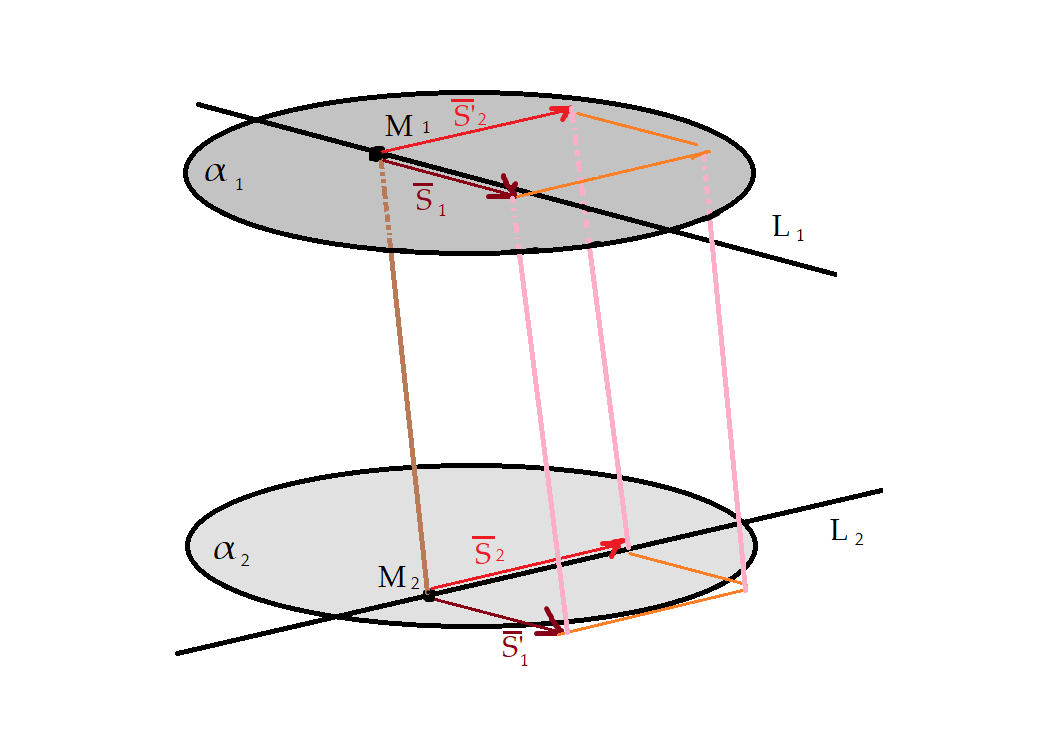
\includegraphics[scale=0.6]{pic11.png}
\end{center}
$L_1$ и $L_2$ скрещиваются, т.е. $\overline{s}_1\,\nparallel\,\overline{s}_2$. Расстояние между прямыми равно высоте параллелепипеда на векторах $\overline{s}_1,\overline{s}_2$ и $\overline{M_1M}_2$.
$$ d(L_1,L_2)=h=\frac{V}{S_{\,\overline{s}_1,\,\overline{s}_2}}=\frac{|\overline{s_1}\cdot\overline{s}_2\cdot\overline{M_1M}_2|}{|\overline{s}_1\times\overline{s}_2|} $$
Если $L_1$ и $L_2$ пересекаются, то $d(L_1,L_2)=0\,\Leftrightarrow\,\overline{s_1}\cdot\overline{s}_2\cdot\overline{M_1M}_2=0\,\Leftrightarrow\,$ $\overline{s}_1,\,\overline{s}_2$ и $\overline{M_1M}_2$ -- компланарны.
\newpage
\subsubsection{Общий перпендикуляр скрещивающихся прямых}
\begin{wrapfigure}{l}{0.5\textwidth}
    \centering
    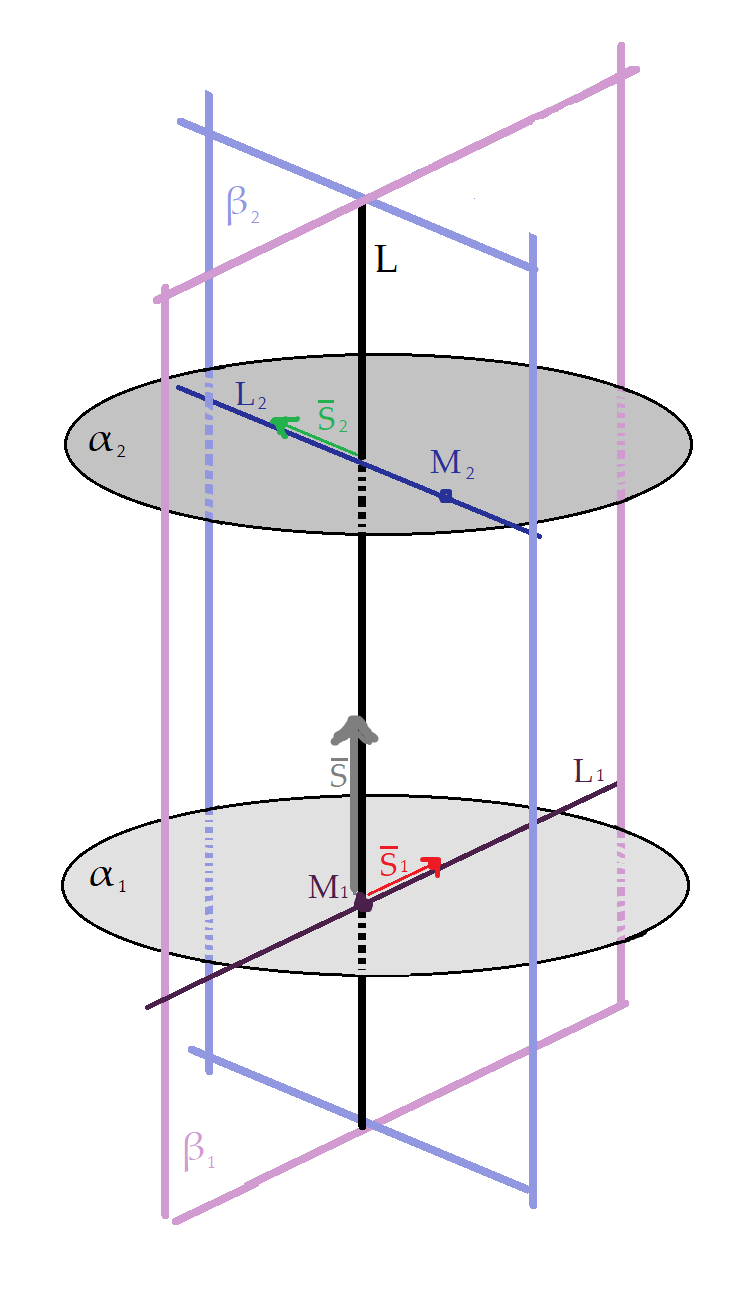
\includegraphics[scale=0.4]{pic12.png}
\end{wrapfigure}
Допустим даны две прямые $L_1$ и $L_2$, их точки $M_1(x_1,y_1,z_1)$ и $M_2(x_2,y_2,z_2)$.

Нужно составить уравнение прямой $L$ -- общего перпендикуляра скрещивающихся прямых $L_1$ и $L_2$.
\begin{enumerate}
    \item Находим координаты векторов $\overline{s}_1=(l_1,m_1,n_1)$ и $\overline{s}_2=(l_2,m_2,n_2)$ -- направляющих векторов прямых $L_1$ и $L_2$.
    \item Находим координаты $(A_1,B_1,C_1)$ вектора нормали $\overline{n}$ плоскости $\alpha_1$, проходящей через прямую $L_1$ параллельно прямой $L_2$, из равенства $\overline{n}=\overline{s}_1\times\overline{s}_2$. Этот вектор будет являться направляющим вектором $\overline{s}$ для искомой прямой $L$.
    \item Проведём плоскость $\beta_1$, в которой лежат прямые $L$ и $L_1$. Её вектор нормали $\overline{n}_1=\overline{s}\times\overline{s}_1$.
    \item Зная координаты точки $M_1(x_1,y_1,z_1)$, принадлежащей прямой $L_1$ и, следовательно, плоскости $\beta_1$, и вектор нормали $\overline{n}_1$, можем составить уранвение плоскости $\beta_1$.
    \item Повторив шаги (2) -- (4), можно составить уравнение плоскости $\beta_2$, проходящей через прямые $L$ и $L_2$.
\end{enumerate}
Прямая $L$ является пересечением плоскостей $\beta_1$ и $\beta_2$ -- система уравнений данных плоскостей будет являться уравнением искомой прямой $L$.

\newpage
\subsection{Задачи о симметричной точке}
\subsubsection{Симметрия относительно прямой}
\textbf{ЗАДАЧА}. Найти координаты точки $M_2(x_2,y_2,z_2)$, симметричной точке $M_1(x_1,y_1,z_1)$ относительно прямой $L\::\: \cfrac{x-x_0}{l}=\cfrac{y-y_0}{m}=\cfrac{z-z_0}{n}$

\textbf{РЕШЕНИЕ}
\begin{enumerate}
    \item Находим уравнение плоскости, которая перпендикулярна данной прямой и проходит через точку $M_1(x_1,y_1,z_1)$. Так как плоскость перпендикулярна заданной прямой, то в качестве ее вектора нормали можно взять направляющий вектор прямой, т.е. $\overline{n}=\overline{s}=(l,m,n)$ Поэтому уравнение плоскости будет иметь вид $\alpha\::\:l(x-x_1)+m(y-y_1)+n(z-z_1)=0$.
    \item Находим точку $M_3(x_3,y_3,z_3)$ пересечения прямой $L$ и плоскости $\alpha$.
    \item Точка $M_3(x_3,y_3,z_3)$ является серединой отрезка $M_1M_2$, где точка $M_2(x_2,y_2,z_2)$ является искомой точкой (duh), поэтому
    $$ \begin{cases}x_2=2x_3-x_1\\y_2=2y_3-y_1\\z_2=2z_3-z_1 \end{cases} $$
\end{enumerate}
\subsubsection{Симметрия относительно плоскости}
\textbf{ЗАДАЧА}. Найти координаты точки $M_2(x_2,y_2,z_2)$, симметричной точке $M_1(x_1,y_1,z_1)$ относительно плоскости $\alpha\::\:Ax+By+Cz+D=0$.

\textbf{РЕШЕНИЕ}
\begin{enumerate}
    \item Находим уравнение прямой, которая перпендикулярна данной плоскости и проходит через точку $M_1(x_1,y_1,z_1)$. Так как прямая перпендикулярна заданной плоскости, то в качестве ее направляющего вектора можно взять вектор нормали плоскости, т.е. $\overline{s}=\overline{n}=(A,B,C)$. Поэтому уравнение прямой будет: $L\::\:\cfrac{x-x_1}{A}=\cfrac{y-y_1}{B}=\cfrac{z-z_1}{C}$.
    \item Находим точку $M_3(x_3,y_3,z_3)$ пересечения прямой $L$ и плоскости $\alpha$.
    \item Точка $M_3(x_3,y_3,z_3)$ является серединой отрезка $M_1M_2$, где точка $M_2(x_2,y_2,z_2)$ является искомой точкой (duh), поэтому
    $$ \begin{cases}x_2=2x_3-x_1\\y_2=2y_3-y_1\\z_2=2z_3-z_1 \end{cases} $$
\end{enumerate}

\newpage
\subsection{Уравнение плоскости через определитель}
Уравнение плоскости можно задать с помощью трёх заданных точек $M_1(x_1,y_1,z_1)$, $M_2(x_2,y_2,z_2)$ и $M_3(x_3,y_3,z_3)$.

Очевидно, что множество точек $M(x,y,z)$ определяет в прямоугольной системе координат $Oxyz$ в трехмерном пространстве плоскость, проходящую через три различные и не лежащие на одной прямой точки $M_1(x_1,y_1,z_1)$, $M_2(x_2,y_2,z_2)$ и $M_3(x_3,y_3,z_3)$ тогда и только тогда, когда три вектора $\overline{M_1M}=(x-x_1,y-y_1,z-z_1)$, $\overline{M_1M}_2=(x_2-x_1,y_2-y_1,z_2-z_1)$ и $\overline{M_1M}_3=(x_3-x_1,y_3-y_1,z_3-z_1)$ компланарны.
\begin{center}
    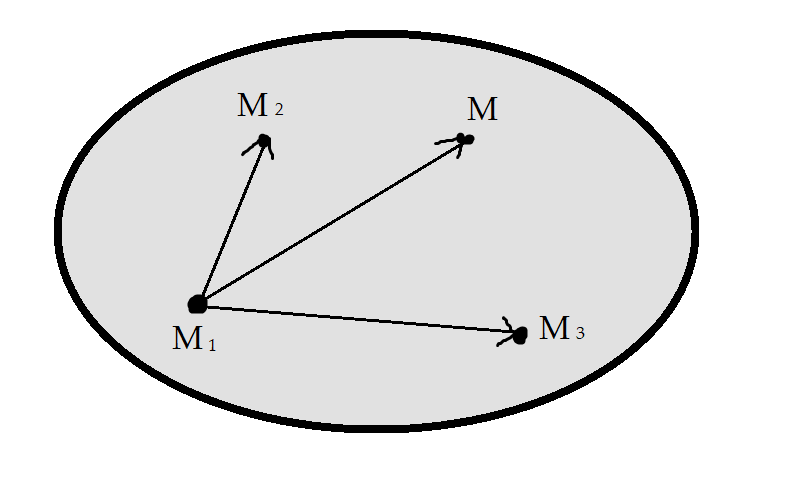
\includegraphics[scale=0.4]{pic13.png}
\end{center}
Следовательно, должно выполняться условие компланарности трех векторов $\overline{M_1M}$, $\overline{M_1M}_2$ и $\overline{M_1M}_3$ -- то есть, их смешанное произведение должно равняться нулю.

\[
    \overline{M_1M}\cdot\overline{M_1M}_2\cdot\overline{M_1M}_3
    =
    \begin{bmatrix}
    x-x_1 & y-y_1 & z-z_1 \\
    x_2-x_1 & y_2-y_1 & z_2-z_1 \\
    x_3-x_1 & y_3-y_1 & z_3-z_1
    \end{bmatrix}
    = 0
    \]
\newpage
\section{Всё про алгебраические кривые второго порядка на плоскости (эллипс, гипербола, парабола).}
\subsection{Табличка}
\begin{center}
\begin{tabular}{ |m{2em}|m{12em}|m{12em}|m{12em}|}
    \hline
     & Эллипс & Гипербола & Парабола \\
    \hline
    \rotatebox{90}{I определение } & 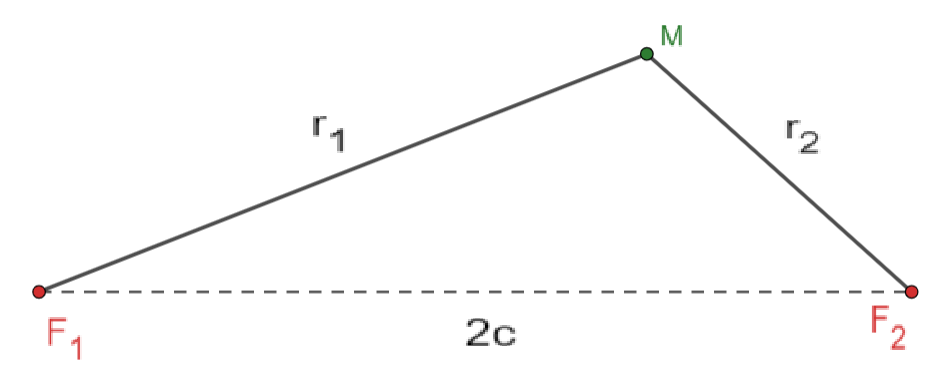
\includegraphics[scale=0.2]{pic14.png} &  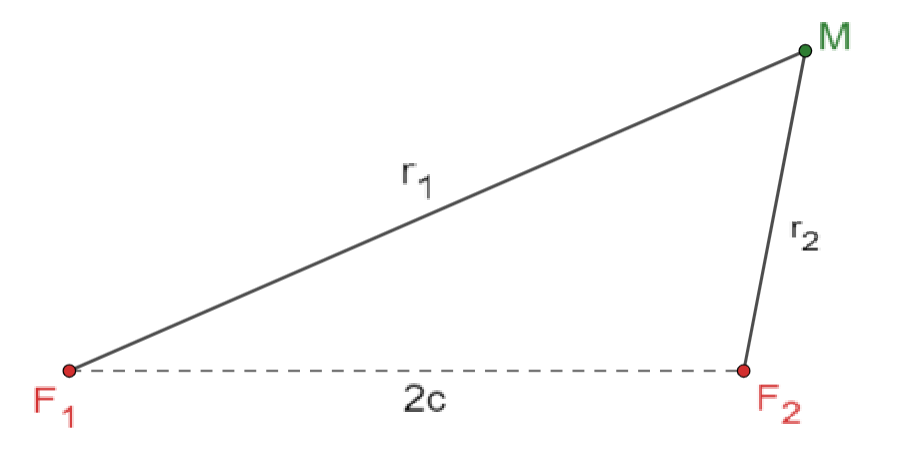
\includegraphics[scale=0.2]{pic15.png} & \begin{center}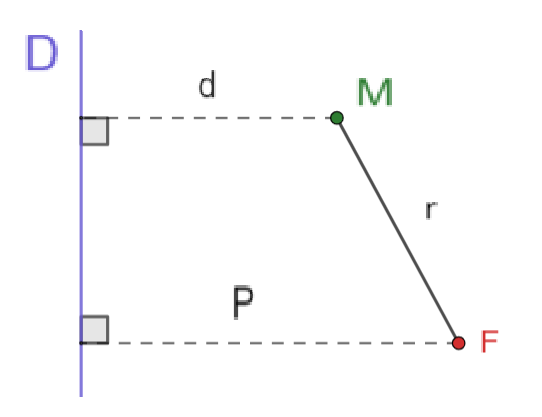
\includegraphics[scale=0.3]{pic16.png}\end{center}\\
    & $$ r_1+r_2=2a>2c $$ $F_1$ и $F_2$ -- фокусы, $r_1$ и $r_2$ -- фокальные радиусы. & $$ |r_2-r_1|=2a<2c $$ $F_1$ и $F_2$ -- фокусы, $r_1$ и $r_2$ -- фокальные радиусы. & $$ r=d $$ $F$ -- фокус, $r$ -- фокальный радиус.\\
    \hline
    \rotatebox{90}{Каноническое $\;\;\;\;$}$\;$ \rotatebox{90}{ уравнение $\;\;\;\;$} & 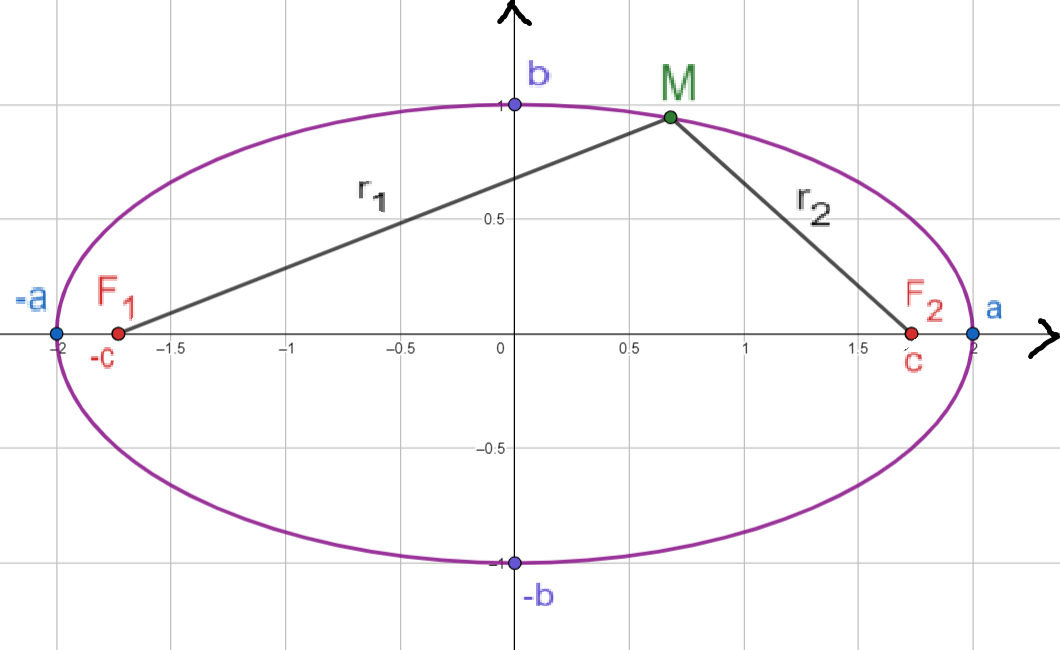
\includegraphics[scale=0.19]{pic17.png} & 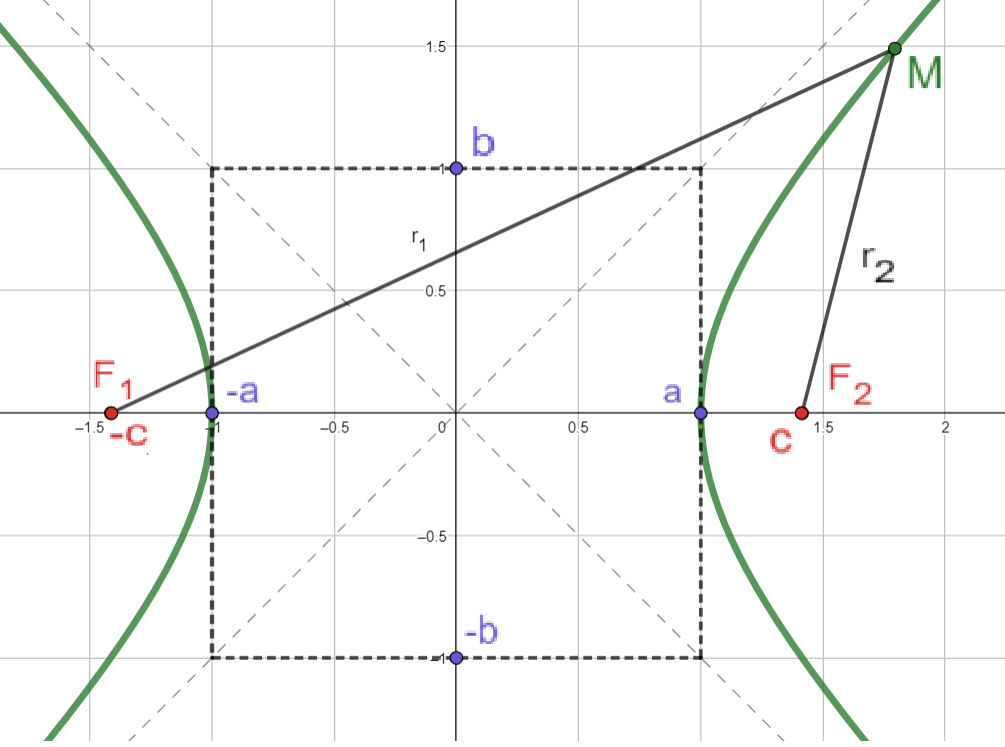
\includegraphics[scale=0.19]{pic18.png} & \begin{center}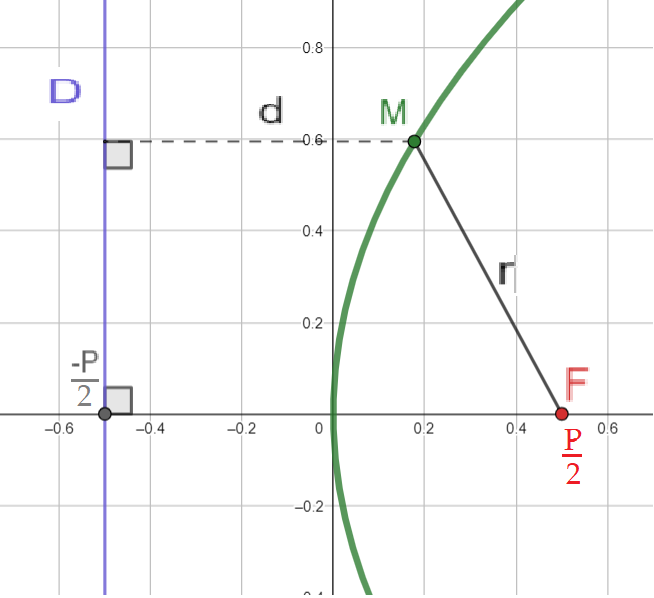
\includegraphics[scale=0.22]{pic19.png}\end{center}\\
    & $$ \frac{x^2}{a^2}+\frac{y^2}{b^2}=1,\,b^2=a^2-c^2 $$ $a$ и $b$ -- большая и малая полуоси. & $$ \frac{x^2}{a^2}-\frac{y^2}{b^2}=1,\,b^2=c^2-a^2 $$ $a$ и $b$ -- действительная и мнимая полуоси. Асимптоты $y=\pm\frac{b}{a}\cdot x$, вершины $a$ и $-a$. & $$ y^2=2Px $$\\
    \hline
    \rotatebox{90}{Эксцен- }$\;$\rotatebox{90}{триситет } & $$ \xi =\frac{c}{a}<1 $$ если $\xi=1$ -- окружность & $$\xi =\frac{c}{a}>1 $$ & $$\xi=1$$\\
    \hline
    \rotatebox{90}{Фокальные }$\;$ \rotatebox{90}{радиусы} & $$ r_{1,2}=a\pm\xi\cdot x $$ & Левая ветвь: $$r_{1,2}=-\xi\cdot x\mp a$$ правая ветвь: $$r_{1,2}=-\xi\cdot x\pm a$$ & $$ r=x+\frac{P}{2} $$\\
    \hline
\end{tabular}
\end{center}
\newpage
\begin{center}
\begin{tabular}{ |m{2em}|m{12em}|m{12em}|m{12em}|}
    \hline
     & Эллипс & Гипербола & Парабола \\
    \hline
    \rotatebox{90}{Директрисы } & 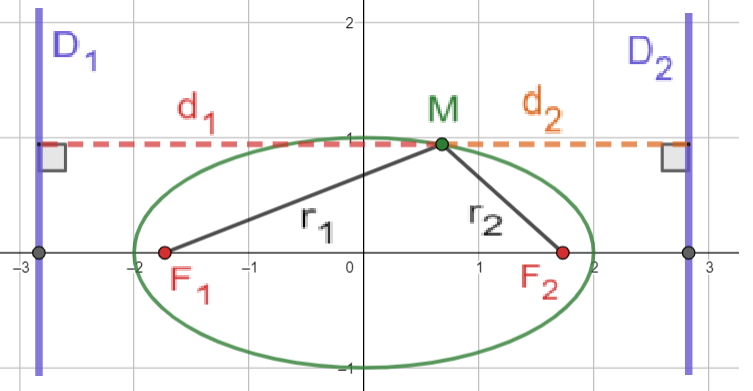
\includegraphics[scale=0.24]{pic20.png} & \begin{center}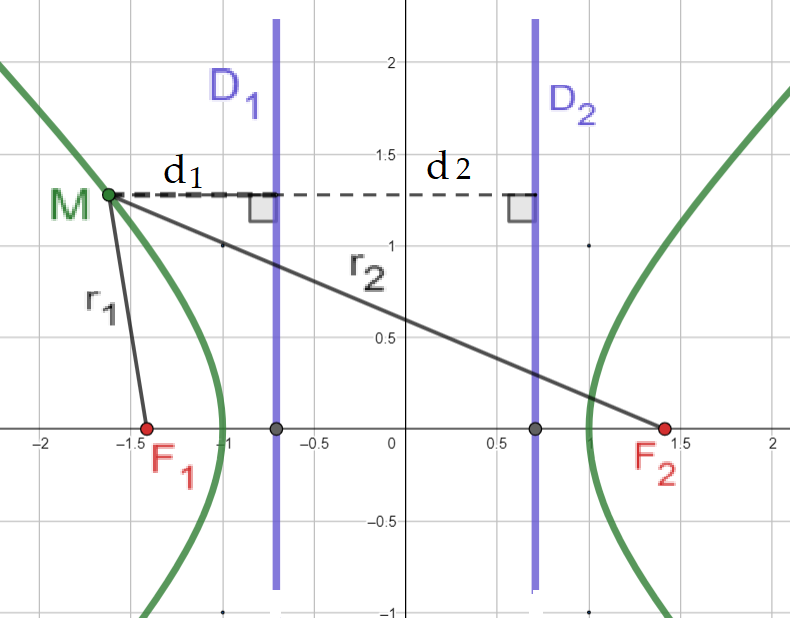
\includegraphics[scale=0.19]{pic21.png}\end{center} & \begin{center}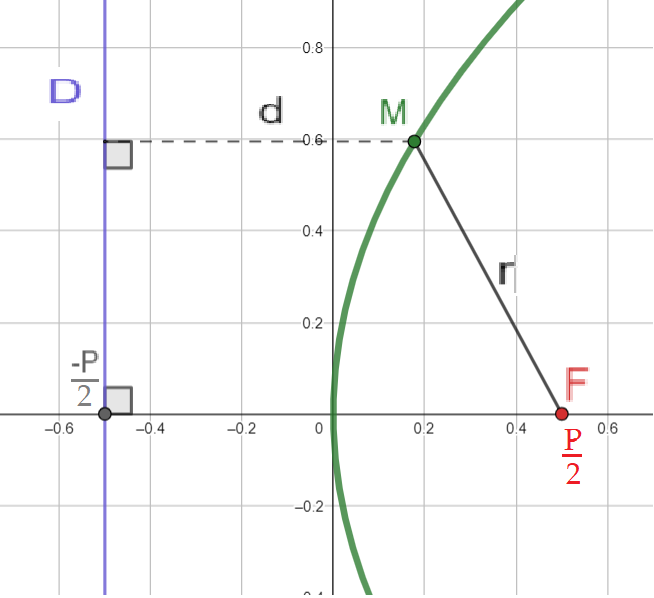
\includegraphics[scale=0.22]{pic19.png}\end{center}\\
    & $$ D_{1,2}\::\: x=\mp\frac{a}{\xi} $$ $$ \frac{r}{d}=\xi=\frac{r_1}{d_1}=\frac{r_2}{d_2} $$ & $$ D_{1,2}\::\:x=\mp\frac{a}{\xi} $$ $$ \frac{r_1}{d_1}=\frac{r_2}{d_2}=\frac{r}{d}=\xi $$ & $$ D\::\:x=-\frac{P}{2} $$ $$ \frac{r}{d}=\xi =1 $$ \\
    \hline
    \rotatebox{90}{II определение $\,$} & 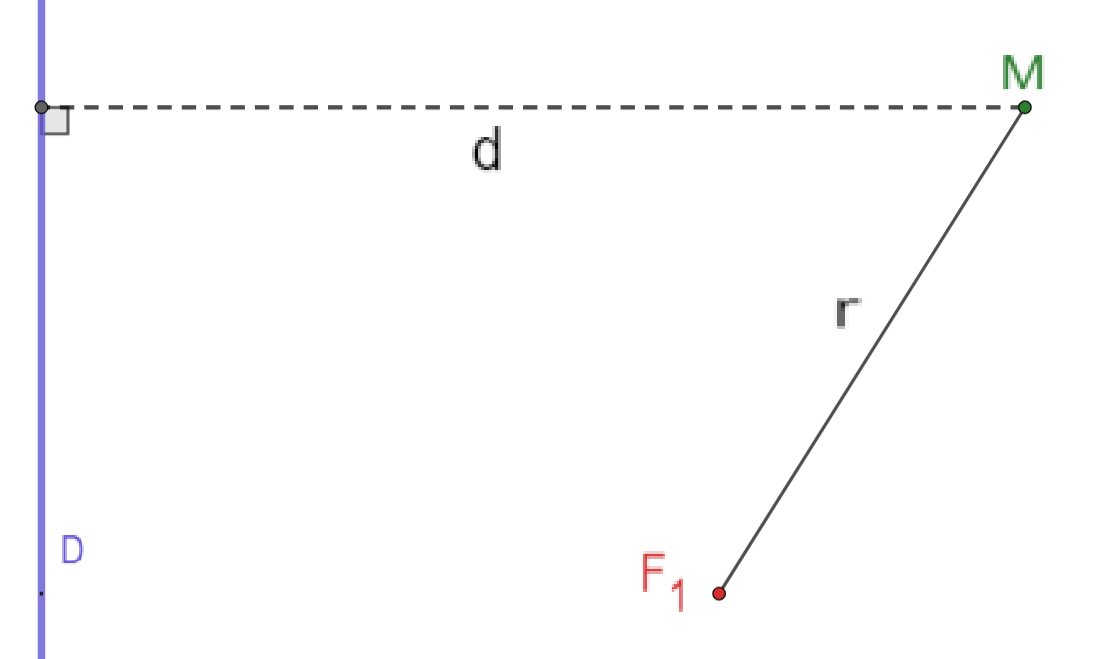
\includegraphics[scale=0.18]{pic22.png} & \begin{center} 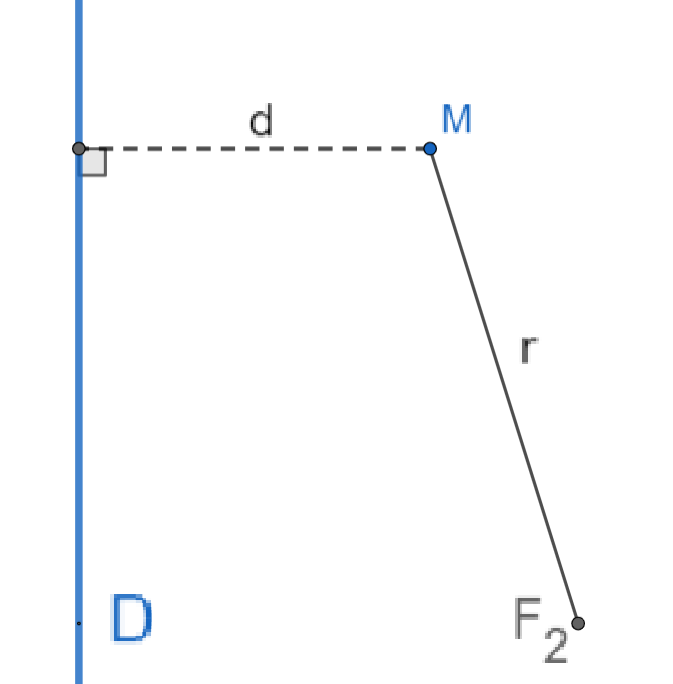
\includegraphics[scale=0.18]{pic23.png} \end{center} & \begin{center} 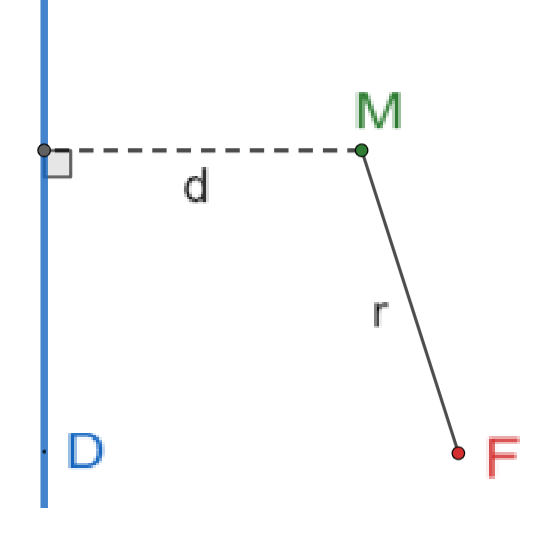
\includegraphics[scale=0.19]{pic24.png} \end{center}\\
    & ГМТ такое, что отношение расстояний от любой из точек до фиксированной точки $F$ и до фиксированной прямой $D$ было меньше $1$. $$ \frac{r}{d}<1 $$ & ГМТ такое, что отношение расстояний от любой из точек до фиксированной точки $F$ и до фиксированной прямой $D$ было больше $1$. $$ \frac{r}{d}>1 $$ & ГМТ такое, что расстояние от любой из точек до фиксированной прямой $D$ было равно расстоянию от любой точки до фиксированной точки $F$. $$ \frac{r}{d}=1 $$\\
    \hline
    & \multicolumn{3}{c|}{а) Начало координат выбирается в фокусе, а полярная ось } \\
    & \multicolumn{3}{c|}{в направлении соответствующей директрисы. $P=\xi\cdot q$ -- фокальный параметр.} \\
    & \multicolumn{3}{c|}{$\;$} \\\cline{2-4}
    \rotatebox{90}{Полярные $\,$}$\;$\rotatebox{90}{уравнения $\,$} & \begin{center} 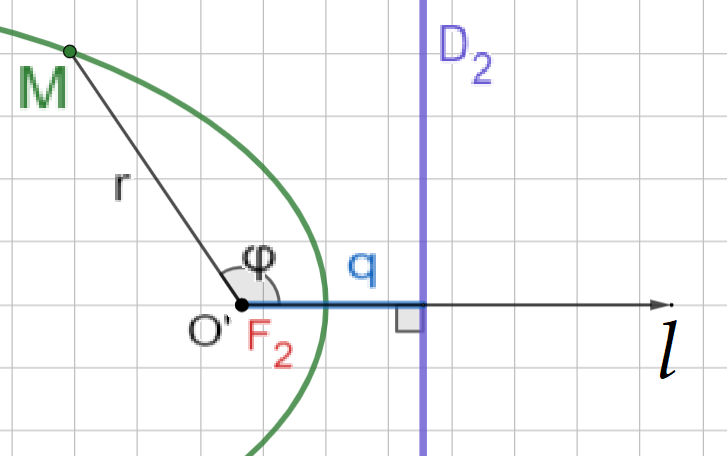
\includegraphics[scale=0.2]{pic25.png} \end{center} & \begin{center} 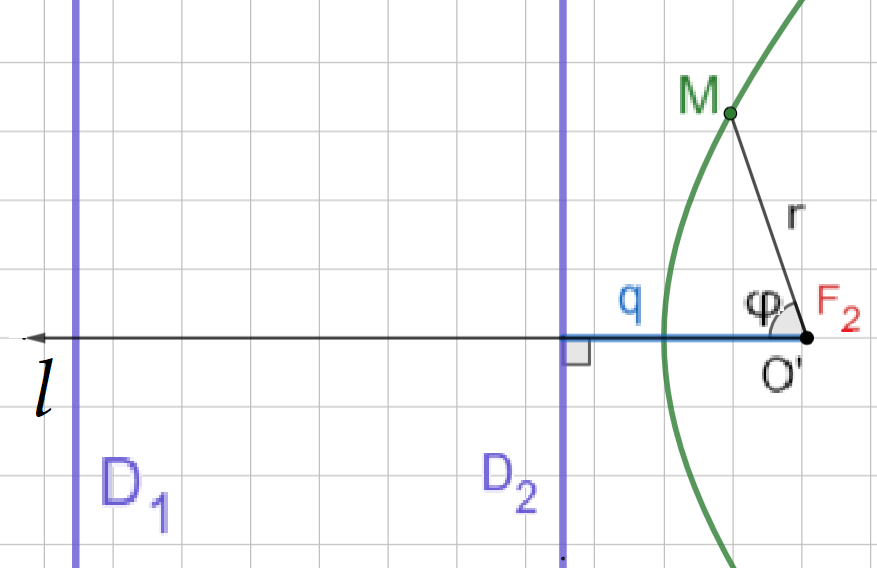
\includegraphics[scale=0.2]{pic26.png} \end{center} & \begin{center} 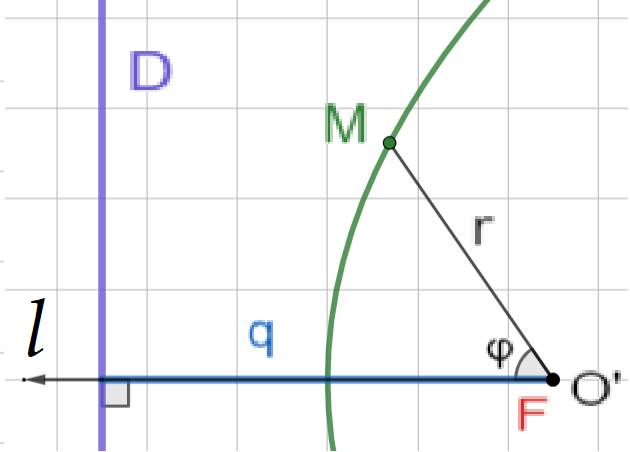
\includegraphics[scale=0.2]{pic27.png} \end{center}\\
    & $$ r=\frac{P}{1+\xi\cos\varphi} $$ $$ P=\frac{b^2}{a}=\xi\cdot(\frac{a}{\xi}-c)=\xi\cdot q $$ & $$ r=\frac{\pm P}{1\pm\xi\cos\varphi} $$ $$ P=\frac{b^2}{a}=\xi\cdot(c-\frac{a}{\xi})=\xi\cdot q $$ & $$ r=\frac{P}{1+\cos\varphi} $$ $$ P=q $$\\
    \hline
\end{tabular}
\end{center}

\newpage
\begin{center}
\begin{tabular}{ |m{2em}|m{12em}|m{12em}|m{12em}|}
    \hline
     & Эллипс & Гипербола & Парабола \\
    \hline
    & \multicolumn{3}{c|}{б) Начало координат выбирается в фокусе, а полярная ось } \\
    & \multicolumn{3}{c|}{в направлении противоположно директрисе. $P=\xi\cdot q$ -- фокальный параметр.} \\
    & \multicolumn{3}{c|}{\textbf{Чё делаем?} Да тупо у тех уравнений выше } \\
    & \multicolumn{3}{c|}{знак меняем в знаменателе на противоположный.} \\
    \hline
    \rotatebox{90}{Уравнение }$\;$\rotatebox{90}{касательной } & \begin{center} 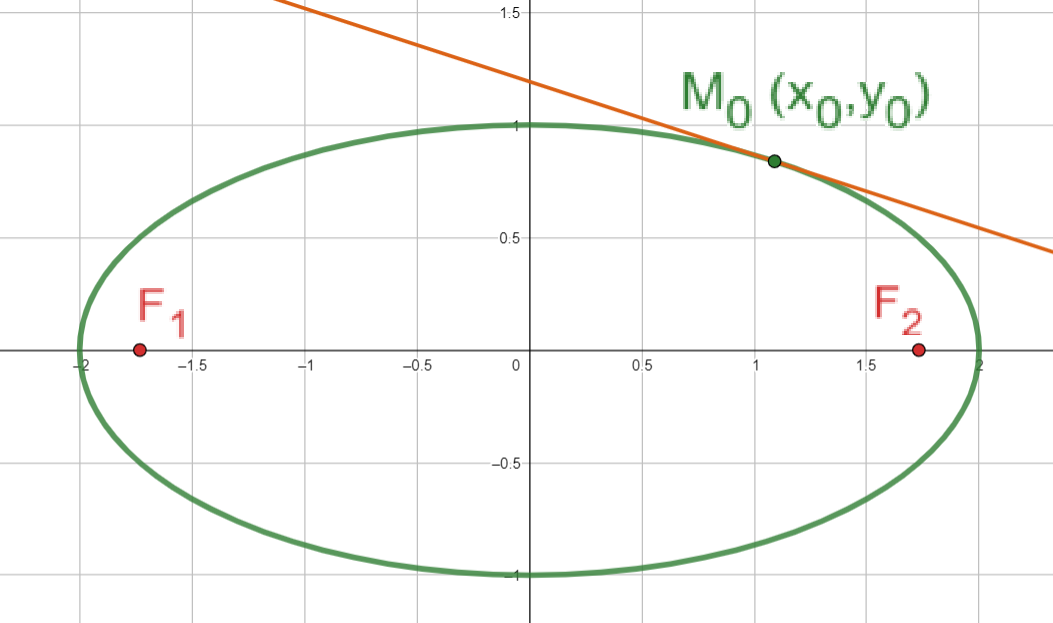
\includegraphics[scale=0.19]{pic28.png} \end{center} & \begin{center} 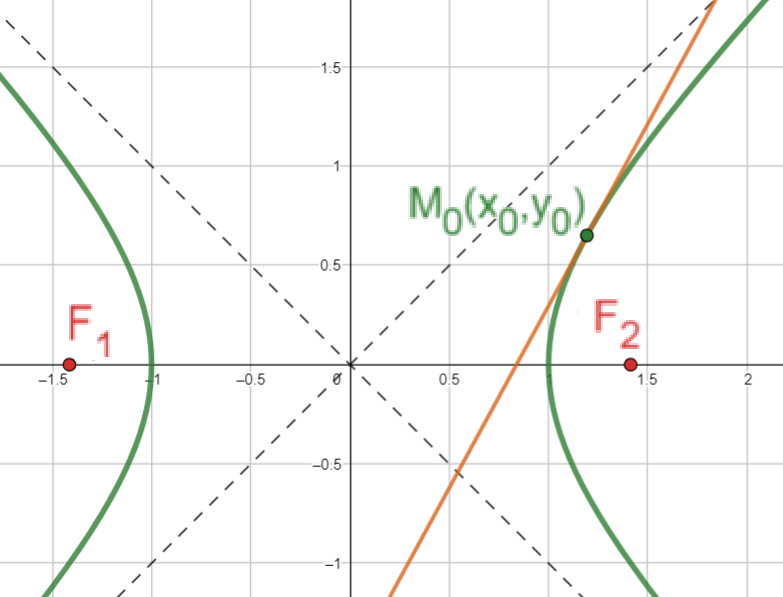
\includegraphics[scale=0.19]{pic29.png} \end{center} & \begin{center} 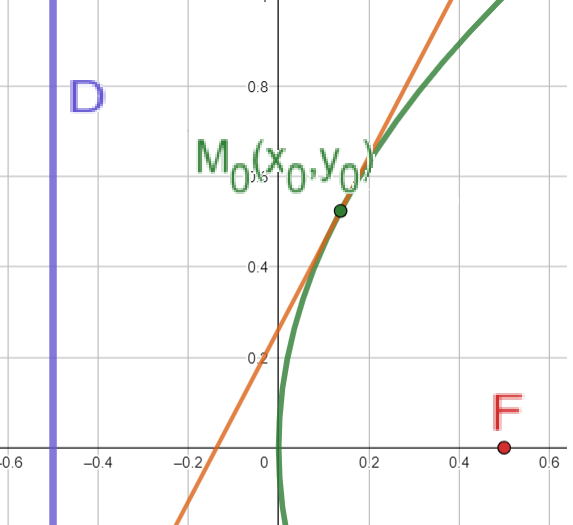
\includegraphics[scale=0.19]{pic30.png} \end{center} \\
    & $$ \frac{xx_0}{a^2}+\frac{yy_0}{b^2}=1 $$ & $$ \frac{xx_0}{a^2}-\frac{yy_0}{b^2}=1 $$ & $$ yy_0=P(x+x_0) $$ \\
    \hline
\end{tabular}
\end{center}
\subsection{Уравнение касательной}
\subsubsection{Уравнение касательной к эллипсу}
\begin{wrapfigure}{l}{0.5\textwidth}
    \centering
    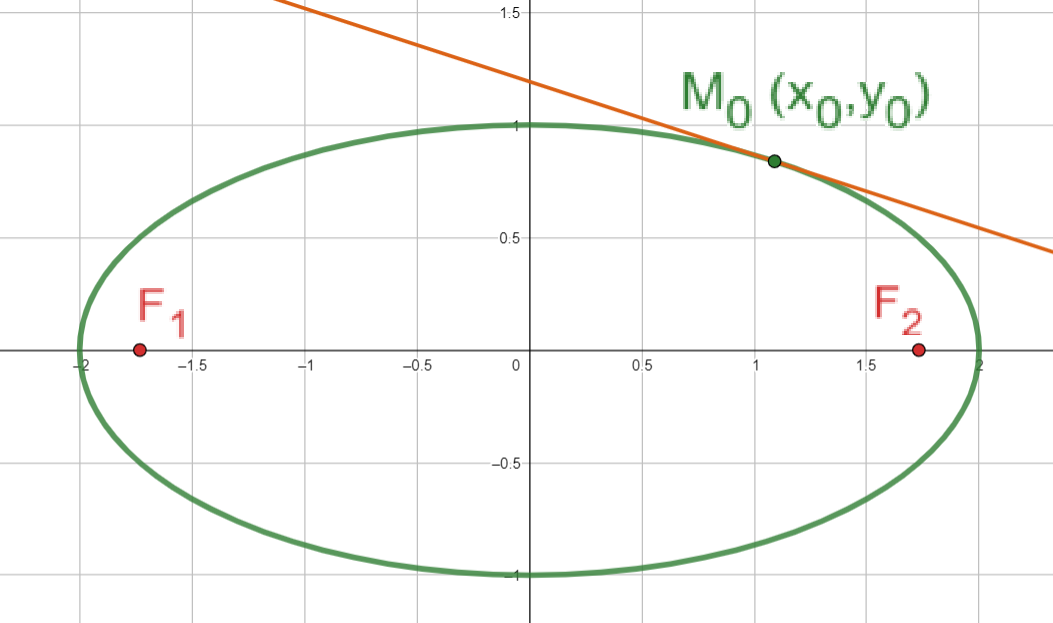
\includegraphics[scale=0.3]{pic28.png}
\end{wrapfigure}
Будем рассматривать для верхней полуплоскости, то есть $x\in(-a;a)$, $y>0$. Уравнение эллипса в таком случае:
$$ y=b\cdot\sqrt{1-\frac{x^2}{a^2}} $$
Уравнение производной в точке $M_0(x_0,y_0)$ (принадлежащей эллипсу):
$$ y-y_0=f'(x_0)(x-x_0) $$
Найдём производную.
$$ y'=b\cdot\cfrac{-\cfrac{2x}{a^2}}{2\cdot\sqrt{1-\cfrac{x^2}{a^2}}}=\cfrac{-bx}{a^2\cdot\sqrt{1-\cfrac{x^2}{a^2}}} $$
$$ y'(x_0)=\cfrac{-bx_0}{a^2\cdot\sqrt{1-\cfrac{x_0^2}{a^2}}}=\cfrac{-bx_0}{a^2\cdot\cfrac{y_0}{b}}=-\frac{b^2x_0}{a^2y_0} $$
Т.к. точка $M_0$ лежит на эллипсе, то уравнение эллипса подходит и для неё, т.е. $y_0=b\cdot\sqrt{1-\cfrac{x_0^2}{a^2}}$. Подставим всю дичь в уравнение касательной.
\newpage
$$ y-y_0=-\frac{b^2x_0}{a^2y_0}\cdot(x-x_0)\,\Leftrightarrow\,a^2y_0(y-y_0)=-b^2x_0(x-x_0)\,\Leftrightarrow $$
$$ \Leftrightarrow\,a^2y_0y-a^2y_0^2=-b^2x_0x+b^2x_0^2\,\Leftrightarrow\,b^2x_0x+a^2y_0y=b^2x_0^2+a^2y_0^2\:\:|\::(a^2b^2)\,\Leftrightarrow$$
$$ \Leftrightarrow\,\frac{x_0x}{a^2}+\frac{y_0y}{b^2}=\frac{x_0^2}{a^2}+\frac{y_0^2}{b^2} $$
Т.к. точка $M_0$ лежит на эллипсе, то $\cfrac{x_0^2}{a^2}+\cfrac{y_0^2}{b^2}=1$, то есть
$$ \frac{x_0x}{a^2}+\frac{y_0y}{b^2}=1 $$

\subsection{Оптические свойства}
\subsubsection{Оптические свойства эллипса}
\begin{wrapfigure}{l}{0.5\textwidth}
    \centering
    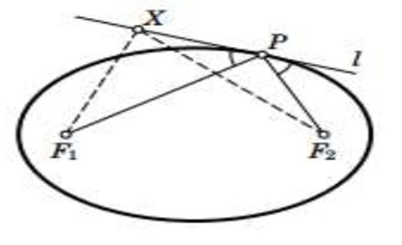
\includegraphics[scale=0.9]{pic31.png}
\end{wrapfigure}
Пусть прямая $l$ касается эллипса в точке $P$, тогда прямая $l$ будет являться внешней биссектрисой угла $F_1PF_2$.

\textbf{Доказательство}
Пусть $X$ -- произвольная точка на прямой $l$, отличная от $P$. Так как $X$ лежит вне эллипса, то
$$ XF_1+XF_2>PF_1+PF_2, $$
т.е. из всех точек прямой $l$ точка $P$ имеет наименьшую сумму расстояний до $F_1$ и $F_2$. \textit{Но какого-то хуя в силу выше сказанного чего-то там бля я не поняла чего, углы бля равны, че бля}

\textbf{Физическая интерпретация}. Если поместить в один из фокусов эллипса с зеркальной "поверхностью" точечный источник света, то все лучи после отражения от этой "поверхности" сойдутся в другом его фокусе.
\begin{center}
    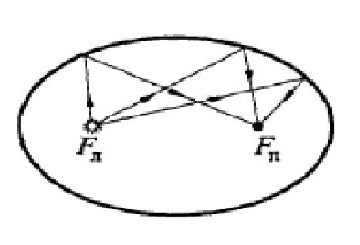
\includegraphics[scale=0.8]{pic32.png}
\end{center}
\newpage
\section{Приведение уравнения кривой второго порядка к каноническому виду.}
Уравнение кривой второго порядка $$ Ax^2+Bxy+Cy^2+2Dx+2Ey+F=0 $$. Если $A$, $B$ и $C$ одновременно не нули -- прямая невырожденная (эллипс, гипербола, парабола), иначе -- вырожденная (пара пересекающихся прямых, пара параллельных прямых,
прямая, точка, пустое множество.)

\begin{enumerate}
    \item $B\neq 0$ -- делаем поворот.

    $$ \begin{cases}x=x'\cos\alpha-y'sin\alpha \\ y=x'\sin\alpha+y'\cos\alpha \end{cases} $$
    Подставляем в уравнение, приравниваем коэффициент при $x'y'$  нулю (то есть коэффициент $B'$), находим косинус и синус угла $\alpha$, подставляем в уравнение, счастливо живем
    \item $B=0$
    \begin{enumerate}
        \item Если $A$ и $C$ не нули одновременно, то выделяем квадраты и анализируем по свободному члену че получается (че)
        \item Если $A\neq0,C=0$, то выделяем квадрат для $x$ и анализируем по свободному члену че получается (че)
        \item Если $A=0,\,C\neq0$, то выделяем квадрат для $y$ и анализируем по свободному члену че получается (че)
    \end{enumerate}
\end{enumerate}
\newpage
\section{Алгебраические поверхности второго порядка. Определение геометрической формы поверхности второго порядка по ее уравнению (метод сечений). Цилиндрические поверхности.}
\subsection{Основные понятия}
\textbf{Алгебраические ПВП} -- ГМТ, координаты которых удовлетворяют алгебраическому уравнению второго порядка.
$$ a_{11}x^2+a_{22}y^2+a_{33}z^2+2a_{12}xy+2a_{13}xz+2a_{23}yz+2a_1x+2a_2y+2a_3z+a_0=0 $$
$$a_{11}^2+a_{22}^2+a_{33}^2+a_{12}^2+a_{13}^2+a_{23}^2\neq0$$
\begin{center}
    \begin{tabular}{|c|c|}
        \hline
        \multicolumn{2}{|c|}{ПВП} \\
        \hline
         Невырожденные & Вырожденные \\
         \hline
         эллипсоид; & точка; \\
         гиперболоид: & прямая; \\
         а) однополостный; & пара $||$ прямых; \\
         б) двуполостный; & пара $\cap$ прямых; \\
         параболоид: & эллиптический цилиндр; \\
         а) эллиптический; & гиперболический цилиндр; \\
         б) гиперболический; & параболический цилиндр; \\
         конус & $\varnothing$; \\
         & плоскость \\
          \hline
    \end{tabular}
\end{center}
\subsection{Метод сечений}

\textit{Я пипец какой ленивый}
\newpage
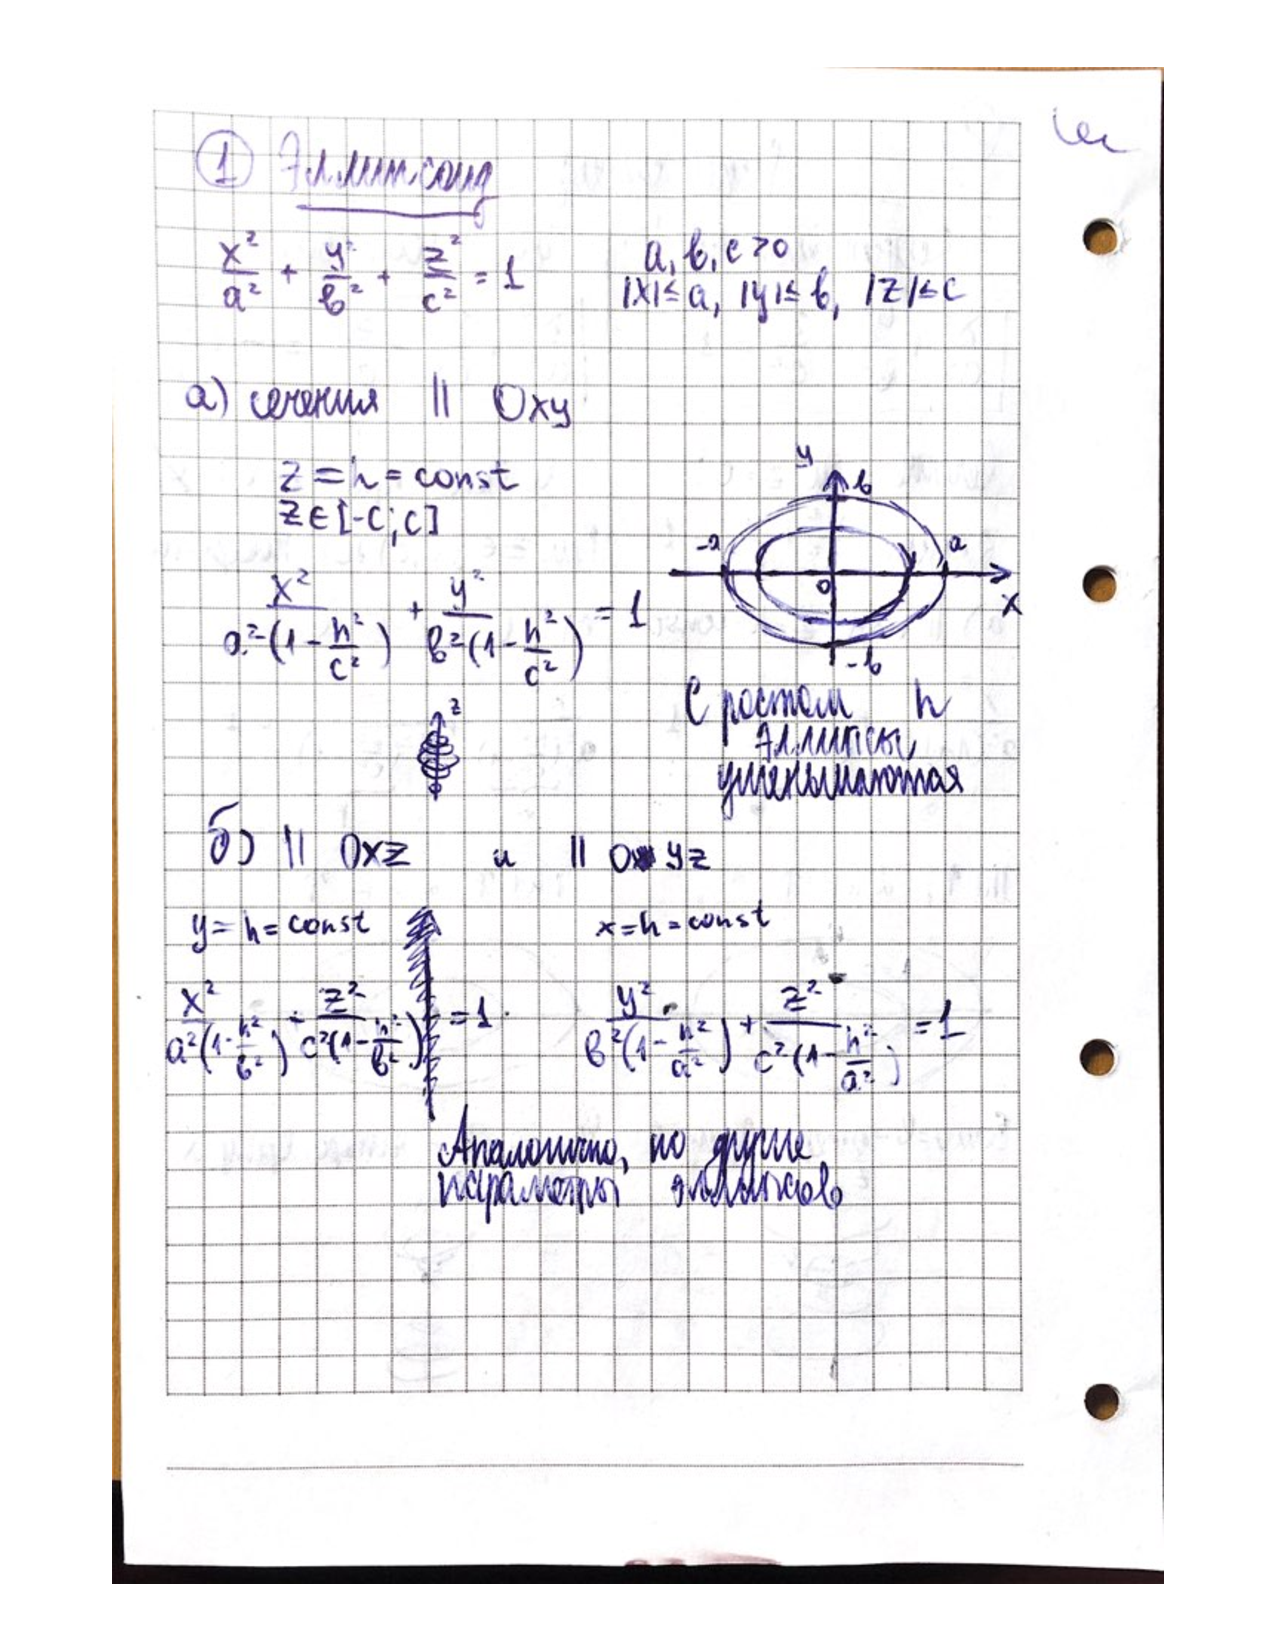
\includepdf[pages=-,pagecommand={},width=\textwidth]{3d.pdf}
\subsection{Цилиндры}
НУ цилиндры это ух как легко, есть там всякие эллиптические (ну как в детстве рисовали), гиперболические (как два бесконечно уходящих в ширину столбика), параболические (один бесконечно уходящий в ширину столбик) и пара пересекающихся плоскостей

еще есть пара параллельных прямых (плоскостей), прямая (плоскость), точка (прямая)

Короч, на плоскости -- какая-то кривая второго порядка, а в пространстве выходит столбик (ну функция $F(x,y)=0$, где $z=0$)
\end{document}
